%========================================
% Plantilla artículo - Humanidades Digitales / NLP
% Compilar con: pdfLaTeX + BibTeX + pdfLaTeX + pdfLaTeX
%========================================
\documentclass[11pt,a4paper]{article}

% --- Codificación y tipografía ---
\usepackage[utf8]{inputenc}   % Si usas LuaLaTeX/XeLaTeX, quita inputenc y usa fontspec
\usepackage[T1]{fontenc}
\usepackage{lmodern}
\usepackage{microtype}

% --- Idioma ---
\usepackage[spanish,es-tabla]{babel}  % "Tabla" en lugar de "Cuadro", etc.
\usepackage{csquotes}

% --- Diseño de página ---
\usepackage[margin=1in]{geometry}
\usepackage{setspace}
%\onehalfspacing  % Activa si quieres interlineado 1.5

% --- Matemáticas y figuras/tablas ---
\usepackage{amsmath,amssymb}
\usepackage{graphicx}
\usepackage{booktabs}
\usepackage{tabularx}
\usepackage{siunitx}
\usepackage{longtable}
\usepackage{array}


% --- Hipervínculos y referencias cruzadas ---
\usepackage[hidelinks,colorlinks=true,linkcolor=blue,citecolor=blue,urlcolor=blue]{hyperref}
\usepackage[nameinlink,capitalise,noabbrev]{cleveref}
\usepackage{float}
\usepackage{subcaption}

% --- Bibliografia ----
\usepackage[round,authoryear]{natbib}
\bibliographystyle{apalike}



% --- Comandos útiles ---
\newcommand{\keywords}[1]{\par\noindent\textbf{Palabras clave —} #1}
\newcommand{\JEL}[1]{\par\noindent\textbf{Clasificación —} #1}
\newcolumntype{P}[1]{>{\centering\arraybackslash}p{#1}}


% --- Metadatos ---
\title{Ciencia en la esfera pública de Colombia: \\
	Análisis del discurso en columnas de opinión con metodologías de humanidades digitales y procesamiento de lenguaje natural}

\author{
	Karen Melissa Gomez Montoya\\
	Biviana Marcela Suárez Sierra\\
	\small Universidad EAFIT, Medellín, Colombia\\
	\small \texttt{tu-email@eafit.edu.co}
}

\date{\today}

%========================================
\begin{document}
	\maketitle
	
	\begin{abstract}
		
	\end{abstract}
	
	\keywords{Humanidades digitales; Análisis del discurso; Procesamiento del lenguaje natural; Opinión pública; Colombia}
	%\JEL{(si aplica)}
	

	\section{Introducción}
	 PENDIENTE TERMINAR
	
	\begin{enumerate}
			
		\item Ciencia en la esfera pública
		
		Sobre la ciencia en la esfera pública, la mayoría de investigaciones se ha enfocado en la confianza hacia ella de la sociedad y en como es comunicada. También se habla de la importancia de la ciencia en debates públicos.
		
		Diversos estudios muestran que la confianza pública tiene muchos beneficios sociales. Por ejemplo \cite{Cologna2025} justifica que facilita que las personas tomen decisiones informadas en salud y nutrición, también ``sienta las bases para la formulación de políticas basadas en la evidencia y facilita el gasto público en investigación.'' 
		
		También se encontró que una alta confianza en la ciencia se correlacionó con mayor aceptación a las vacunas en la pandemia por Covid-19 \cite{Sturgis2021}. También si las personas no creen en el cambio climático no contribuirían siguiendo las medidas para frenar su avance.
		
		A nivel demográfico, algunos factores asociados a una mayor confianza en la ciencia son: ser mujer, tener mayor edad, residir en zonas urbanas, poseer ingresos altos, tener educación formal, profesar una religión y ubicarse en posiciones ideológicas de izquierda \cite{Cologna2025}.
		
		La manera en que se habla de la ciencia, científicos y organizaciones científicas en los medios tiene un papel importante en la confianza de la sociedad en la ciencia. \cite{Mede2022} encuentra que en algunos países los medios tradicionales pueden fortalecer  la confianza en la ciencia y los científicos, aliviando actitudes anticientíficas, pero en otros países los medios fomentan estas actitudes. 
		
		\cite{Donois2025} analizan artículos publicados en el periódico que tratan temas controvertidos relacionados a las ciencias: Cambio climático, vacunas y organismos genéticamente modificados, para encontrar representaciones de la ciencia y los científicos en los medios.  Identificaron cuatro temas relevantes en el discurso tanto de los periodistas como de los comentarios a los artículos: \\
		Tema 1. Clasifican a los científicos como ``verdaderos'' o como ``pseudocientíficos''. \\
		Tema 2. Científicos como héroes o villanos según sus motivos. Héroes cuando se considera que buscan el bien común y salvar personas. O villanos, cuando son vistos como arrogantes, con el deseo de reemplazar a dios o faltos de ética.\\
		Tema 3. Ciencia vs naturaleza y el saber popular. También existe dualidad en este discurso. La ciencia que busca proteger a la naturaleza versus la ciencia que busca superar a la naturaleza o que es incrédula frente a la sabiduría popular, e incluso es retratada como dañina para las personas.\\
		Tema 4. Rechazo al saber científico por motivos de confianza, ideología o falta de debate.
		
		\cite{Donois2025} expresan también que "la investigación sobre cómo los periodistas y sus lectores perciben a los científicos que trabajan y comunican sobre ciencia controvertida sigue siendo escasa, pues la mayoría de los estudios se ha centrado en la confianza en la ciencia y la experticia"
		
		 \cite{Peer2025} argumenta la importancia de la participación de los científicos en los debates públicos, en particular aquellos que impliquen la creación y adopción de políticas públicas medio ambientales. E incluso se promueve que en los parlamentos haya asesoramiento científico, \cite{SantillnGarca2021} 
		 describen los mecanismos de asesoramiento científico los cuales generan espacios de confluencia entre decisores de políticas públicas y expertos científicos, argumentado la importancia de estos.
		 
		 \item Ciencia en la esfera pública colombiana
		 
		 Percepción
		 Comunicación
		 Asociaciones
		 
		 Para las organizaciones del ecosistema Ciencia, Tecnología e Innovación (CTeI) en
		 Colombia, tanto nacionales como regionales, es de vital importancia monitorear la
		 percepción que los ciudadanos tienen sobre la ciencia \cite{Daza_Caicedo2014}.
		 Conocer lo que los colombianos piensan acerca de la ciencia permite a estas
		 organizaciones mejorar los procesos de apropiación social del conocimiento,
		 movilizar agendas políticas y académicas, evaluar las estrategias comunicativas e
		 identificar los imaginarios sociales que circulan en la esfera pública alrededor de la
		 actividad científica \cite{Daza_Caicedo2014}. 
		 
		 Una de las estrategias que se ha usado en Colombia para monitorear dicha
		 percepción han sido las encuestas nacionales. En Colombia se han aplicado tres en
		 diferentes años con el fin de evaluar cómo percibe el ciudadano el ámbito científico:
		 en 1994 la primera, luego en 2004 y por último la aplicada por el Observatorio
		 6
		 Colombiano de Ciencia y Tecnología en el 2012 \cite{Daza_Caicedo2014}
		 
		 \item Columnas de opinión y esfera pública
		 
		 Sobre las columnas de opinión. Estudio hecho sobre columnas de opinión colombianas. Ideas tomadas de \cite{CaroLopera2020}.
		 
		 \begin{itemize}
		 	\item ``Los medios de actualidad no reflejan la realidad tal cual es, sino que la construyen desde una determinada perspectiva.''
		 	\item Se da ``la construcción de representaciones de la realidad de acuerdo con intereses de actores sociales y políticos.''
		 	\item ``El género discursivo de la columna de opinión, al servicio del periodismo, recoge
		 	una amplia tradición histórica en la cual prevalece su condición argumentativa.''
		 	\item Usualmente tratan temas actuales y se redactan con libertad expresiva
		 	\item ``en las columnas se trata de extraer datos de la realidad periodística o de sus vivencias y
		 	pasarlos por la propia ideología, vestida con un lenguaje intimista y de libertad expresiva.''
		 	\item ``el locutor (ethos) apela a las emociones de los receptores (pathos), con un contenido reflexivo o conocimiento comunicado (logos) que apunta a la eficacia persuasiva de convencer.''
		 	\item En las columnas de opinión, se hace uso de estrategias argumentativas para persuadir al lector de ideas.
		 	\item También se mencionan los tipos de argumentos encontrados más comunes: Pragmático, causa-efecto, autoridad, lo probable. 
		 \end{itemize}
		 
		 \cite{Coppock2018} encuentran que las columnas de opinión pueden persuadir y alterar la perspectiva u opiniones de quienes lo leen, sean personas de elite o del público general.
		 
		 En ocasiones, científicos eligen como medio de comunicación escribir columnas de opinión. Al respecto \cite{Syfert2025} encuentran que los cientificos a menudo no tienen la suficiente retórica para convencer a lectores a cambiar sus opiniones a pesar de las pruebas científicas que expresan, a menudo escriben más para personas que ya tienen una opinión similar. 
		
		
		\item Pregunta de investigación
		
		
		A partir de este contexto, la presente investigación busca responder:
		¿Con qué temas, organizaciones, actores y eventos se asocia la ciencia en las columnas de opinión en Colombia, y qué patrones discursivos emergen de estas asociaciones?
		
		Para responder esta pregunta el objetivo es aplicar métodos de humanidades digitales y procesamiento de lenguaje natural en un corpus que consiste en más de 13 mil columnas de opinión publicadas entre 2018 y 2020 en tres periódicos colombianos de alta circulación. 
		
		Los métodos para resolver ....
		
		\item Humanidades digitales ??
		
		
		\item Análisis de discurso basado en NLP
		
		
		\item Este paper se organiza así ...
	\end{enumerate}


	
	\section{Metodología}
	
	Para responder a la pregunta de investigación propuesta, se aplicaron métodos de minería de texto y procesamiento de lenguaje natural (PLN). La metodología se dividió en tres partes principales: Primero, identificar menciones a la ciencia en las columnas de opinión y crear un subcorpus. Luego, aplicar algoritmos para analizar los autores, los actores, temas y vocabulario tanto en el subcorpus como en el corpus general para hacer comparaciones. Y, por último, interpretar los elementos obtenidos a la luz de acontecimientos ocurridos en el país durante las fechas de publicación de las columnas de opinión, además de identificar afiliaciones de autores y actores mencionados para enriquecer el análisis. 
	El proceso realizado se describe en el diagrama de flujo...
	Todos estos análisis se llevaron a cabo en Python. 
	
	\subsection{Diagrama de flujo}
	
	Preprocesamiento básico -> Descriptivos textos -> Bertopic texto -> Fragmentar texto -> Búsqueda ciencia -> Análisis ciencia -> Descriptivos -> Bertopic -> Entidades
	
	\subsection{Recolección data}
	???
	Se recolectaron 13 mil columnas de opinión de tres periódicos colombianos de alta circulación. Estas fueron publicadas entre enero de 2018 y diciembre de 2020.  En esta fase el único filtro de selección fue que la columna fuera completamente texto y no incluyera video o audio necesario para entender su contenido. Las columnas no se seleccionaron por ningún tema en especifico.
	
	Para cada columna de opinión se recolectaron los siguientes metadatos: el nombre del periódico, el autor, la fecha, el título, el texto (cuerpo) de la columna y el vínculo. Se verificó que cada texto sea único (las columnas no se repiten) y se normalizaron los nombres de los autores. Luego de este proceso de asignaron números de identificación únicos para columna de opinión. 
	
	\subsection{Preprocesamiento}
	
	Cuando se analiza texto, es necesario prepararlo y limpiarlo para llevarlo a un formato adecuado antes de aplicar los algoritmos de PLN \cite{Chai2022}. A esta etapa se le conoce como preprocesamiento del texto.  En esta investigación, primero se efectuó una limpieza en el texto de cada columna de opinión, eliminando las urls, los hashtags y las menciones a usuarios de redes sociales (@), así como espacios en blanco extra y caracteres distintos de letras, números y puntuación común. Luego se aplicaron diversas técnicas como tokenización, eliminación de stopwords y lematización según la necesidad de cada algoritmo de análisis. Estas técnicas se definen y explican a continuación. \\
	
	La tokenización es el proceso mediante el cual un texto se divide en unidades más pequeñas llamadas tokens. Este paso permite transformar el texto no estructurado en un formato estructurado y, por tanto, susceptible de análisis \cite{Tyagi_text}. En este trabajo, la tokenización se realizó dividiendo el texto por espacios, es decir, segmentándolo en palabras. \\
	
	Las stopwords son palabras muy frecuentes en el idioma que contribuyen a la coherencia en la construcción de frases, pero que a menudo aportan poco significado para los análisis realizados mediante algoritmos de PLN \cite{Siino2024}. Por ello, es común eliminarlas en etapas previas del procesamiento. Además, los límites computacionales y de tiempo hacen deseable reducir el número de palabras a analizar. Las stopwords son específicas para cada lengua y suelen pertenecer a categorías gramaticales como preposiciones, pronombres, adverbios, artículos y conjunciones \cite{Siino2024}. Los programas de procesamiento de lenguaje suelen incluir listas predefinidas de stopwords, las cuales deben revisarse y pueden ajustarse según las necesidades del estudio. En este trabajo, las stopwords fueron eliminadas antes del modelado de tópicos. \\
	
	
	La lematización implica reducir las palabras a su forma básica o raíz, lo que se conoce como lema, lo que ayuda a estandarizar el uso de las palabras en todo el texto. Por ejempo, lleva los verbos a infinitivo y las palabras en plural a singular \cite{Orellana2018}. Esta técnica es especialmente importante para tareas como el análisis de frecuencia de términos. La elección del modelo adecuado de lematización es fundamental. El primer criterio a considerar es el idioma del texto analizado, posteriormente, es necesario verificar que los resultados obtenidos sean correctos. En esta investigación, la lematización se aplicó antes del análisis léxico y el POS-tagging. Inicialmente se usó el algoritmo de lematización de la librería spaCy de Python, que aunque es rápido, no tuvo la precisión requerida. Finalmente, se usó el algoritmo de Stanford Stanza \cite{qi2020stanza}, que produjo resultados más precisos. 
	
	
	\subsection{Identificación de menciones a la ciencia}
	Para alcanzar el objetivo propuesto en esta investigación, es necesario identificar las menciones a la ciencia presentes en un texto. Para ello, se desarrolló una estrategia derivada de la búsqueda semántica, utilizada como método de recuperación de información. La búsqueda semántica permite la recuperación de resultados o documentos basándose en la similitud semántica sin que haya superposición de palabras clave \cite{Wei2022}. Para lograrlo, combina embeddings, que son representaciones vectoriales de los textos que preservan significado y contexto, con métodos para medir la similitud semántica, como la similitud de coseno. \\
	
	
	
	En este trabajo se empleó, como representación vectorial de los textos, un modelo de embeddings de oraciones basado en la arquitectura transformer. Esta arquitectura permite que los modelos aprendan el contexto en ambas direcciones para una palabra o frase. En particular, se utilizó Sentence-BERT (S-BERT) \cite{reimers-2019-sentence-bert, reimers-2020-multilingual-sentence-bert}, el cual ha demostrado ser eficiente y eficaz en tareas de similitud semántica medidas mediante la similitud de coseno. Específicamente, se empleó un modelo multilingüe que incluye el español: sentence-transformers/paraphrase-multilingual-MiniLM-L12-v2 [REF]. Este modelo fue elegido porque .. 
	
	La métrica que se usó para evaluar la similaridad entre los textos luego de ser codificados a embeddings fue la similitud de coseno. Para dos vectores $\mathbf{u}$ y $\mathbf{v}$ se define como:
	
	\begin{equation}
		\text{sim}_{\cos}(\mathbf{u}, \mathbf{v}) = 
		\frac{\mathbf{u} \cdot \mathbf{v}}
		{\|\mathbf{u}\| \, \|\mathbf{v}\|}
	\end{equation}
	
	donde $\mathbf{u} \cdot \mathbf{v}$ es el producto punto entre los vectores, y 
	$\|\mathbf{u}\|$ y $\|\mathbf{v}\|$ corresponden a las normas euclidianas de cada uno \cite{Jurafsky2025}. Su valor oscila entre 1 y -1. Siendo 1 cuando los vectores van en la misma dirección, 0 si son perpendiculares y -1 cuando van en direcciones opuestas. \\
	
	

	
	Para realizar las búsquedas semánticas en el texto de las columnas de opinión, todo los textos fueron divididos en fragmentos o ``chunks'', de tamaño 300 palabras con un mínimo de 100 palabras. Elegir un mínimo es importante, ya que cada columna se dividió en los trozos empezando desde la primera palabra. Luego fue posible que el último trozo de cada columna quedara demasiado corto. En caso de que el ultimo trozo no sea mayor al mínimo definido este se unió al trozo anterior.
	
	
	La razón para dividir fragmentos es que en común las columnas de opinión traten diferentes temas en el texto que es columnas de opinión  es que en textos muy largos puede ser complicado detectar menciones a la ciencia por todos los otros temas que podrían encontrarse, y en muy cortos se pierde el contexto necesario. También se aplica solapamiento entre los chunks, esto es que el segundo chunk de una columna no empieza exactamente cuando termina el otro si no un poco antes, esto facilita no perder contexto. 
	Luego para cada chunk se calculará el embedding representativo.

	\subsubsection{Tesauro de la UNESCO}
	¿Cómo podemos encontrar menciones y referencias a la ciencia en los fragmentos? Implementaremos búsqueda del tipo semántica. Para este tipo de búsqueda no es tan útil una definición de ciencia como un conjunto de términos que construyan un campo semántico especifico. Para esto se propone utilizar el tesauro de la UNESCO en la categoría ciencia.  
	¿Por qué usar este tesauro? El tesauro de la UNESCO ``es una lista controlada y estructurada de términos para el análisis temático y la búsqueda de documentos y publicaciones en los campos de la educación, cultura, ciencias naturales, ciencias sociales y humanas, comunicación e información.'' \cite{unesco_thesaurus_1977}. 
	Su primera versión en inglés fue publicada en 1977 pero es revisado y actualizado periódicamente. Para este trabajo usaremos en particular la lista llamada Ciencia, especializada en ciencias naturales. Esta lista nos permite acercarnos a la ciencia a partir de las palabras que la componen o se usan para identificarla en diferentes áreas. Esta categoría está compuesta por 17 subcategorías y cada una de ellas contiene entre 24 y 84 términos.
	Para referencia, se incluye una tabla con los primeros términos de cada categoría en \ref{tab:categorias_ciencia}.
	
	
	
	{\footnotesize
		\begin{longtable}{p{3.5cm}P{2cm}p{9cm}}
			\caption{Categorías de Ciencia del Tesauro de la UNESCO y los primeros términos de cada una.} \label{tab:categorias_ciencia}\\
			
			\toprule
			\textbf{Categoría} & \textbf{Nº de términos} & \textbf{Primeros 10 términos} \\
			\midrule
			\endfirsthead
			
			\multicolumn{3}{c}{{\bfseries \tablename\ \thetable{} -- continuación}} \\
			\toprule
			\textbf{Categoría} & \textbf{Nº de términos} & \textbf{Primeros 10 términos} \\
			\midrule
			\endhead
			
			\midrule \multicolumn{3}{r}{{Continúa en la siguiente página}} \\
			\endfoot
			
			\bottomrule
			\endlastfoot
			
			Enfoque científico & 50 & Análisis causal, Análisis comparativo, Análisis cualitativo, Análisis cuantitativo, Análisis de inspección, Análisis transnacional, Autoevaluación, Calibración, Causa y efecto, Ciencia de la ciencia \\
			
			Administración de la ciencia y de la investigación & 62 & Academia de ciencias, Actividad científica, Administración de la ciencia, Ambientalista, Automatización, Brecha digital, Cambio tecnológico, Centro de investigación, Ciencia y desarrollo, Científico \\
			
			Matemáticas y estadística & 34 & Álgebra, Algoritmo, Análisis de regresión, Análisis de variancia, Análisis estadístico, Análisis factorial, Análisis funcional, Análisis matemático, Análisis multivariado, Análisis numérico \\
			
			Ciencias físicas & 56 & Acústica, Aerodinámica, Calefacción, Calor, Congelación, Conversión de energía, Corriente de agua, Cristalografía, Difusión, Dinámica de fluidos \\
			
			Ciencias químicas & 50 & Acido, Análisis bioquímico, Análisis cromatográfico, Análisis de oligoelementos, Análisis espectroquímico, Análisis químico, Azufre, Carbono, Cinética química, Combustión \\
			
			Ciencias del espacio & 24 & Actividad solar, Agujero negro, Astrofísica, Astronomía, Ciencias del espacio, Cosmología, Espacio, Espacio intersideral, Estrellas, Galaxia \\
			
			Ciencias de la tierra & 61 & Arena, Biogeoquímica, Calor terrestre, Ciencias de la tierra, Conservación del suelo, Corteza terrestre, Cuaternario, Datos geológicos, Depósito de sal, Deriva de los continentes \\
			
			Geografía y oceanografía & 84 & Agua de mar, Aguas costeras, Alta mar, Arrecife de coral, Batimetría, Biogeografía, Biología marina, Carta batimétrica, Ciencia del desierto, Circulación oceánica \\
			
			Meteorología & 34 & Agroclimatología, Atmósfera, Bioclimatología, Ciclo hidrológico, Ciclón, Circulación atmosférica, Clima, Climatología, Condiciones metereológicas, Control meteorológico \\
			
			Hidrología & 46 & Abastecimiento de agua, Agua, Agua del suelo, Agua dulce, Agua potable, Agua salada, Agua salobre, Agua subterránea, Agua superficial, Almacenamiento de agua \\
			
			Ciencias ambientales e ingeniería & 52 & Abastecimiento de energía, Alcantarillado, Aprovechamiento de recursos, Balance energético, Calidad ambiental, Ciencias ambientales, Conservación ambiental, Conservación de la fauna y flora silvestres, Conservación de la energía, Conservación de la naturaleza \\
			
			Polución, catástrofes y seguridad & 54 & Accidente, Adaptación al cambio climático, Agua residual, Alud, Asistencia por desastre, Calentamiento de la tierra, Cambio climático, Contaminación, Contaminación atmosférica, Contaminación del agua \\
			
			Recursos naturales & 53 & Adaptación biológica, Biogás, Bioma, Biomasa, Biosfera, Comportamiento animal, Consumo alimenticio, Crisis ecológica, Diversidad biológica, Ecología animal \\
			
			Biología & 75 & Anatomía, Aparato respiratorio, Bacteria, Bacteriología, Bioética, Biofísica, Biogénesis, Biología, Biología celular, Biología espacial \\
			
			Ciencias naturales & 50 & Alga marina, Animal, Animal acuático, Animal de laboratorio, Animal doméstico, Animal marino, Animal salvaje, Antropología, Árbol, Ave \\
			
			Ciencias médicas & 54 & Acupuntura, Aparato sensorial, Ciencias médicas, Cirugía, Control de alimentos, Dietética, Economía de la salud, Endocrinología, Epidemiología, Estadísticas sanitarias \\
			
			Patología & 40 & Cáncer, Ceguera, Daltonismo, Deficiencia mental, Enfermedad, Enfermedad cardiovascular, Enfermedad de la piel, Enfermedad del sistema nervioso, Enfermedad mental, Enfermedad nutricional \\
			
		\end{longtable}
	}
	
	
	%% UNESCO: https://skos.um.es/unescothes/view.php?l=es&fmt=1
	
	%% https://vocabularies.unesco.org/documents/thesaurusintrospa.pdf
	
	
	
	
	Por cada subcategoría, se calculará un embedding representativo. Eso se hará calculando el embedding respectivo a cada término de la subcategoría y luego promediando todos.
	
	Luego se calculará la similitud de coseno para cada embedding de cada fragmento de columna con cada embedding de subacategoría para encontrar cercanía  semántica. Este valor se encuentra entre -1 y 1, donde un número más alto indica mayor similaridad semántica. Usualmente el valor es mayor a cero. Luego se requiere encontrar un umbral que permita separar los fragmentos suficientemente cercanos para clasificar como mención a la ciencia.
	
	\subsubsection{Umbral de selección}
	
	Para encontrar un umbral que permita maximizar la diferencia entre lo que se determina como una mención de ciencia, de lo que no, primero se calculará la similaridad de coseno entre los embeddings de cada fragmento y cada subcategoría de términos. 
	
	Se consideran inicialmente, al observar la distribución, las similaridades mayores a 0.3. Luego por cada categoría se selecciona aleatoriamente un subconjunto de los fragmentos que cumplen esa similaridad. Este subconjunto es clasificado por un ser humano como mención de ciencia o no. Luego el conjunto construido debe ser de un tamaño pequeño: 7 fragmentos por cada subcategoría para un total de 119 textos, que se garantiza sean todos diferentes y que cada uno se compara con la categoría en la tiene mayor valor (mayor similaridad).
	
	Para determinar el umbral que logra la precisión más alta, se calcula para diferentes valores de umbrales, desde 0 hasta 1, en un salto de 0.01, la cantidad de aciertos de cada umbral según la clasificación hecha por humanos. 
	
	Con este umbral se seleccionan los fragmentos que se consideran menciones de ciencia. 
	
	\[
	\mathbf{S} =
	\begin{bmatrix}
		s_{1,1} & s_{1,2} & s_{1,3} & \cdots & s_{1,n} \\
		s_{2,1} & s_{2,2} & s_{2,3} & \cdots & s_{2,n} \\
		s_{3,1} & s_{3,2} & s_{3,3} & \cdots & s_{3,n} \\
		\vdots  & \vdots  & \vdots  & \ddots & \vdots  \\
		s_{m,1} & s_{m,2} & s_{m,3} & \cdots & s_{m,n}
	\end{bmatrix}
	\]
	
	\[
	\text{donde } s_{i,j} = \text{similitud}( \text{Texto}_i, \text{C	at}_j )
	\]
	
	\[
	\mathbf{S} =
	\begin{array}{c|ccccc}
		& \text{cat}_1 & \text{cat}_2 & \text{cat}_3 & \cdots & \text{cat}_n \\ \hline
		\text{Texto}_1 & 0.92 & 0.46 & 0.12 & \cdots & 0.77 \\
		\text{Texto}_2 & 0.88 & 0.51 & 0.09 & \cdots & 0.69 \\
		\text{Texto}_3 & 0.73 & 0.60 & 0.15 & \cdots & 0.81 \\
		\vdots         & \vdots & \vdots & \vdots & \ddots & \vdots \\
		\text{Texto}_m & 0.55 & 0.33 & 0.28 & \cdots & 0.91
	\end{array}
	\]
	
	
	\subsection{Análisis descriptivos y exploratorios de textos y autores}
	\subsection{Análisis de entidades – NER}
	Con el modelo Babelscape/wikineural-multilingual-ner \cite{tedeschi-etal-2021-wikineural-combined}, que se encuentra en la librería Sentence Transformers, se hará un reconocimiento de entidades, entre los textos que tienen menciones de ciencia. Este modelo es capaz de hacer reconocimiento de entidades en texto en español. Reconoce lugares, personas, organizaciones y los demás elementos que considera entidades pero no clasifica entre los anteriores grupos los asigna a miscelaneos. 
	
	\subsection{Análisis de temas}
	\subsection{Análisis léxico-discursivo/ vocabulario (keywords in context, concordancias, n-grams, POS-tagging)}
	
	

	
	\section{Resultados}
	
	En esta sección ...
	Nueva estructura:
	a.	Preprocesamiento ¿Cuántas palabras quedaron luego del preprocesamiento? ¿Qué diferencia hay entre el texto crudo y el texto procesado?
	b.	Identificación menciones a la ciencia. 
	i.	Umbral y valor de accuracy
	ii.	 ¿Cuántas quedaron después? Algunos ejemplos.
	iii.	Por subcategorías
	c.	Análisis descriptivos y exploratorios de textos y autores (comparativos)
	i.	Estadísticos descriptivos generales del corpus vs ciencia
	ii.	Distribución de columnas y autores por periódico, general vs ciencia
	iii.	Nubes de palabras general vs ciencia
	iv.	Distribución temporal general vs ciencia
	v.	Top autores en ciencia vs top en corpus
	vi.	Por subcategorías
	d.	Análisis de entidades – NER (comparativos)
	i.	Tabla con metadatos? 
	ii.	Resumen por afiliación
	iii.	Resumen organización, actores, lugar
	iv.	Top 
	e.	Análisis de temas (comparativos)
	i.	Temas obtenidos
	ii.	
	f.	Análisis léxico-discursivo/ vocabulario (keywords in context, concordancias, n-grams, POS-tagging) (comparativos)
	
	
	\subsection{Análisis exploratorio y estadisticos descriptivos del corpus}
	Las columnas de opinión reunidas provienen de tres periodicos colombianos: El Espectador, El Tiempo, El Colombiano, desde Enero de 2018 a Diciembre de 2020. 
	
	\begin{table}[H]
		\centering
		\caption{Estadísticos descriptivos generales del corpus}
		\label{tab:estadisticos_generales}
		\begin{tabular}{l c}
			\hline
			\textbf{Estadístico} & \textbf{Valor} \\
			\hline
			Número total de documentos & 13676\\
			Palabras totales & 8607473\\
			Promedio palabras por documento & 629\\
			Mediana palabras por documento & 590\\
			Máximo palabras por documento & 5223\\
			Mínimo palabras por documento & 128\\
			Número de autores distintos & 584\\
			Número de periódicos distintos & 3\\
			Número de palabras únicas (vocabulario total) & 283923\\
			\hline
		\end{tabular}
	\end{table}
	
	La riqueza léxica obtenida como el cociente entre el total de palabras únicas y el total de palabras fue del 3.3\%.
	
	
	\begin{table}[H]
		\centering
		\caption{Distribución de columnas y autores por periódico}
		\label{tab:col_autores_periodico}
		\begin{tabular}{l c c c}
			\hline
			\textbf{Periódico} & \textbf{Número de columnas} & \textbf{Número de autores distintos} & \textbf{\% del total de columnas} \\
			\hline
			El Tiempo & 10509 & 263 & 76.84\\
			El Espectador & 1982 &  249 & 14.49\\
			Semana & 1185 & 96  & 8.66\\
			\hline
		\end{tabular}
	\end{table}
	
	\begin{figure}[H]
		\centering
		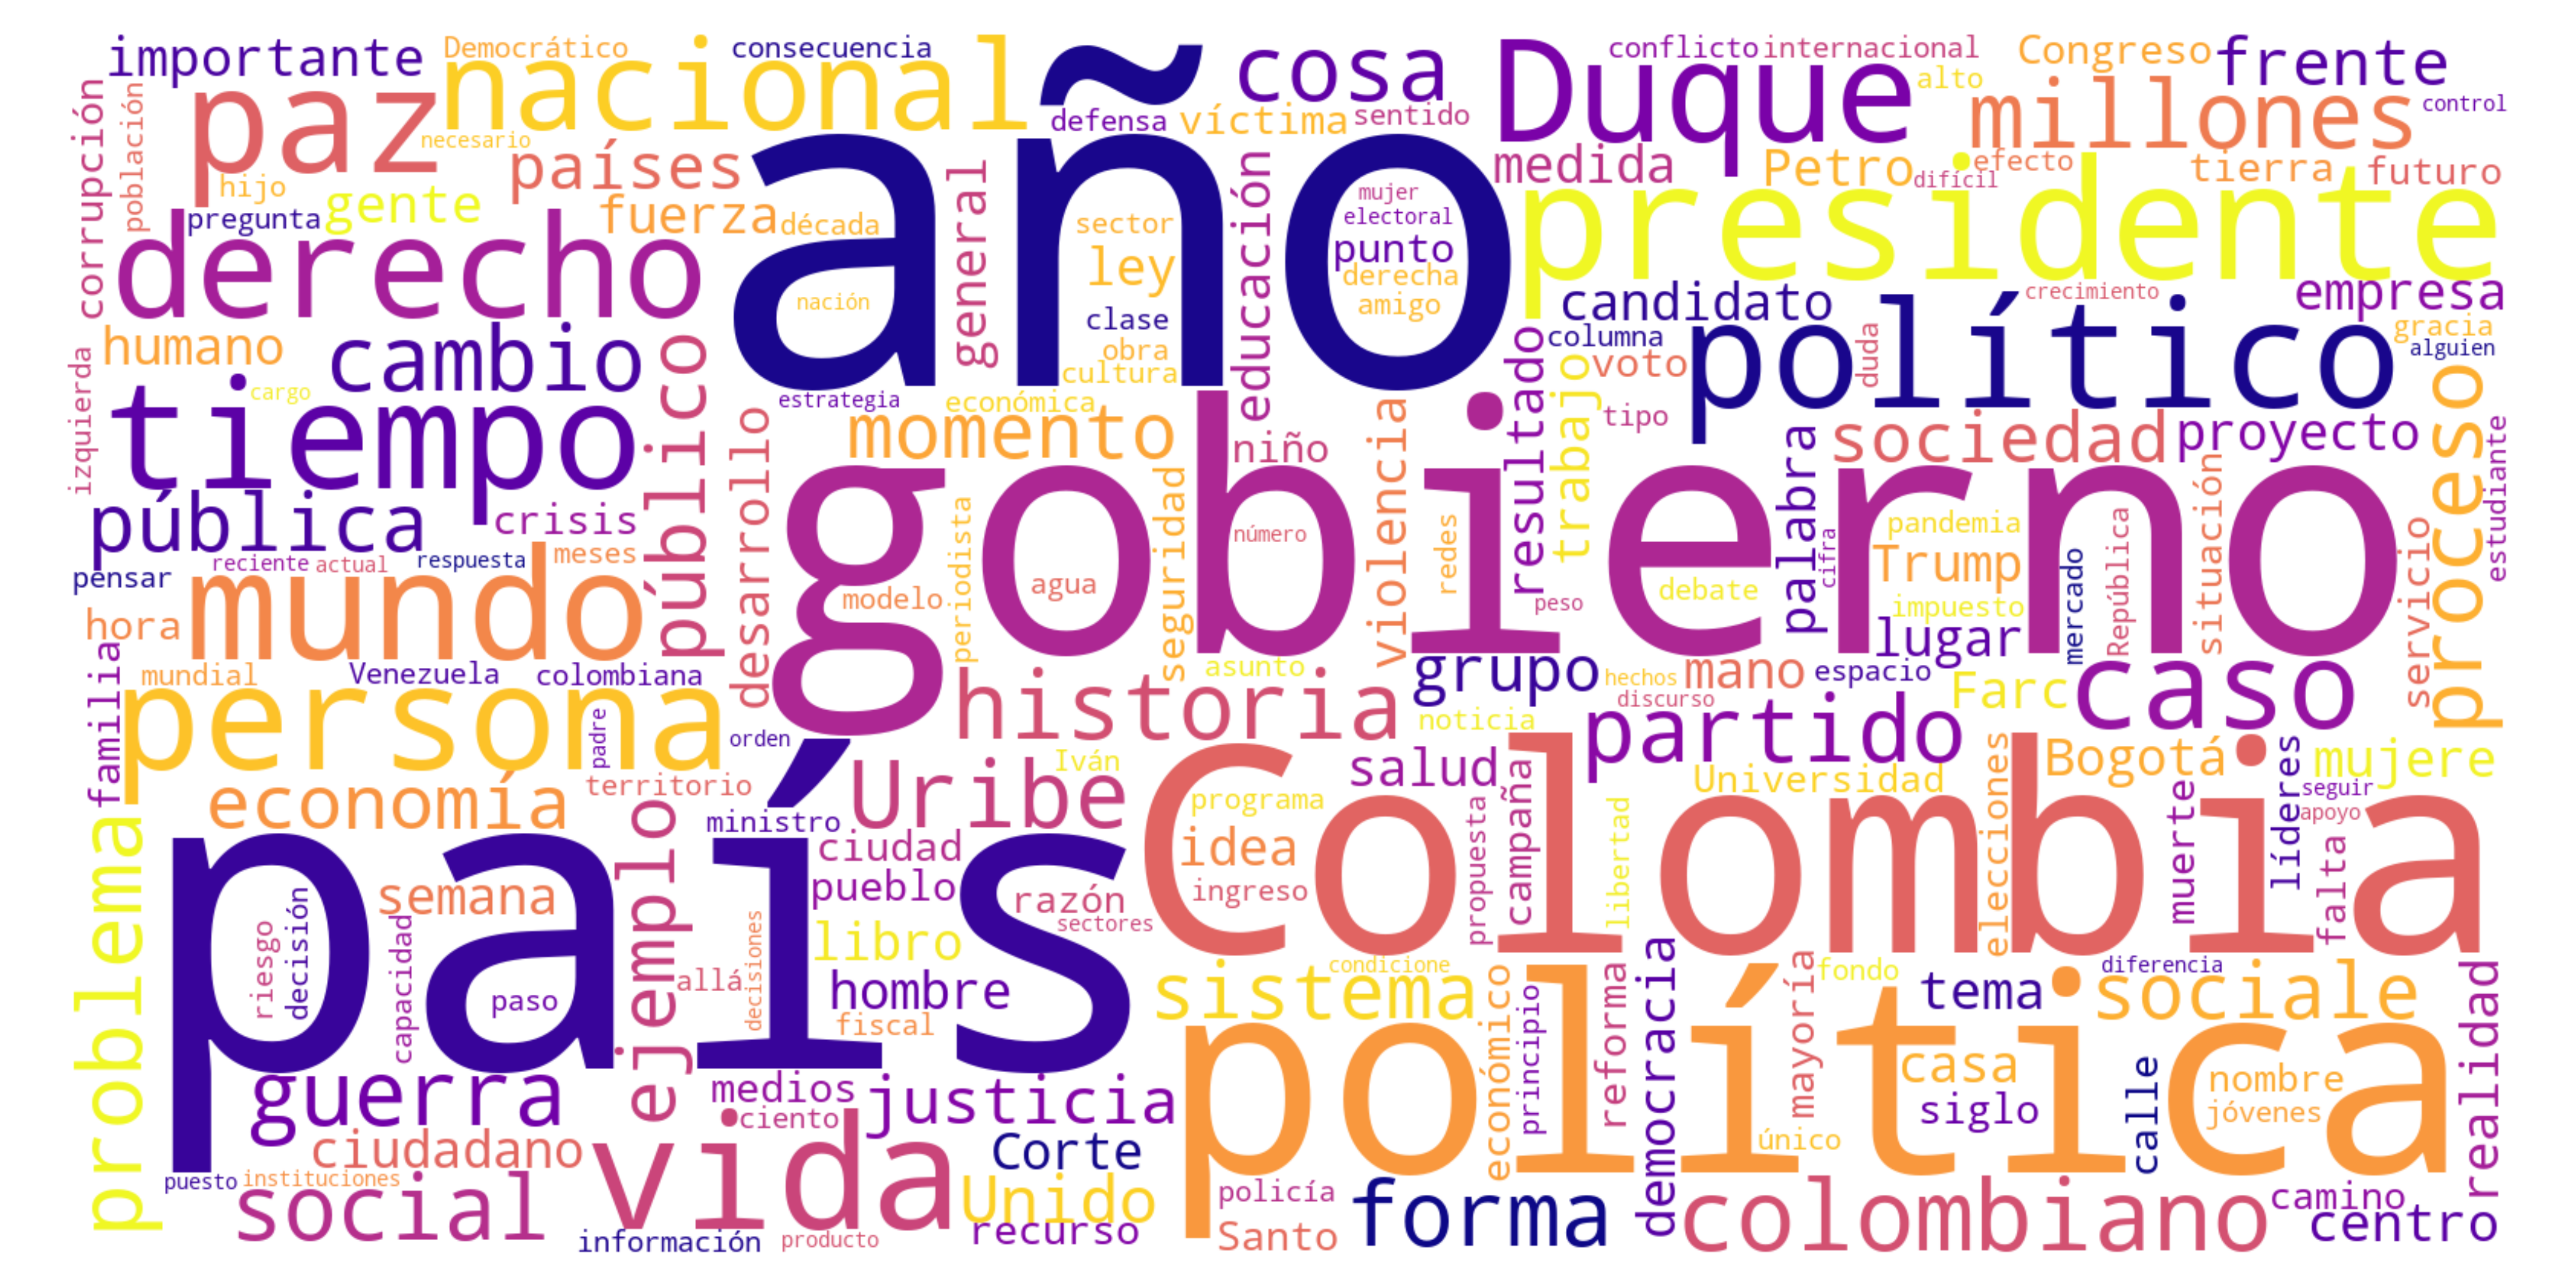
\includegraphics[width=0.9\textwidth]{figures/nube_palabras.png}
		\caption{Nube de palabras del corpus general (sin stopwords)}
		\label{fig:nube-palabras}
	\end{figure}
	
	\subsection{Elección umbral para búsqueda de ciencia}
	 En la Figura \ref{fig:distribucion-scores}, se encuentra la distribución de scores dados por la similaridad de coseno, para cada uno de los fragmentos previamente etiquetados como ciencia o no ciencia. No en todos los casos, mayores valores de score implica que el fragmento está más relacionado con ciencia pero si la mayoría de veces, luego permite estimar. 
	 Al calcular el accuracy para cada umbral entre 0 y 1 con paso 0.01, se encuentra que el valor que mejor separa las dos clases es el 0.40, Figura \ref{fig:accuracy-umbral}.
	
	\begin{figure}[H]
		\centering
		\begin{subfigure}{0.48\textwidth}
			\centering
			
\includegraphics[width=\textwidth]{figures/distribucion_scores.png}
			\caption{Distribución de scores.}
			\label{fig:distribucion-scores}
		\end{subfigure}
		\hfill
		\begin{subfigure}{0.48\textwidth}
			\centering
			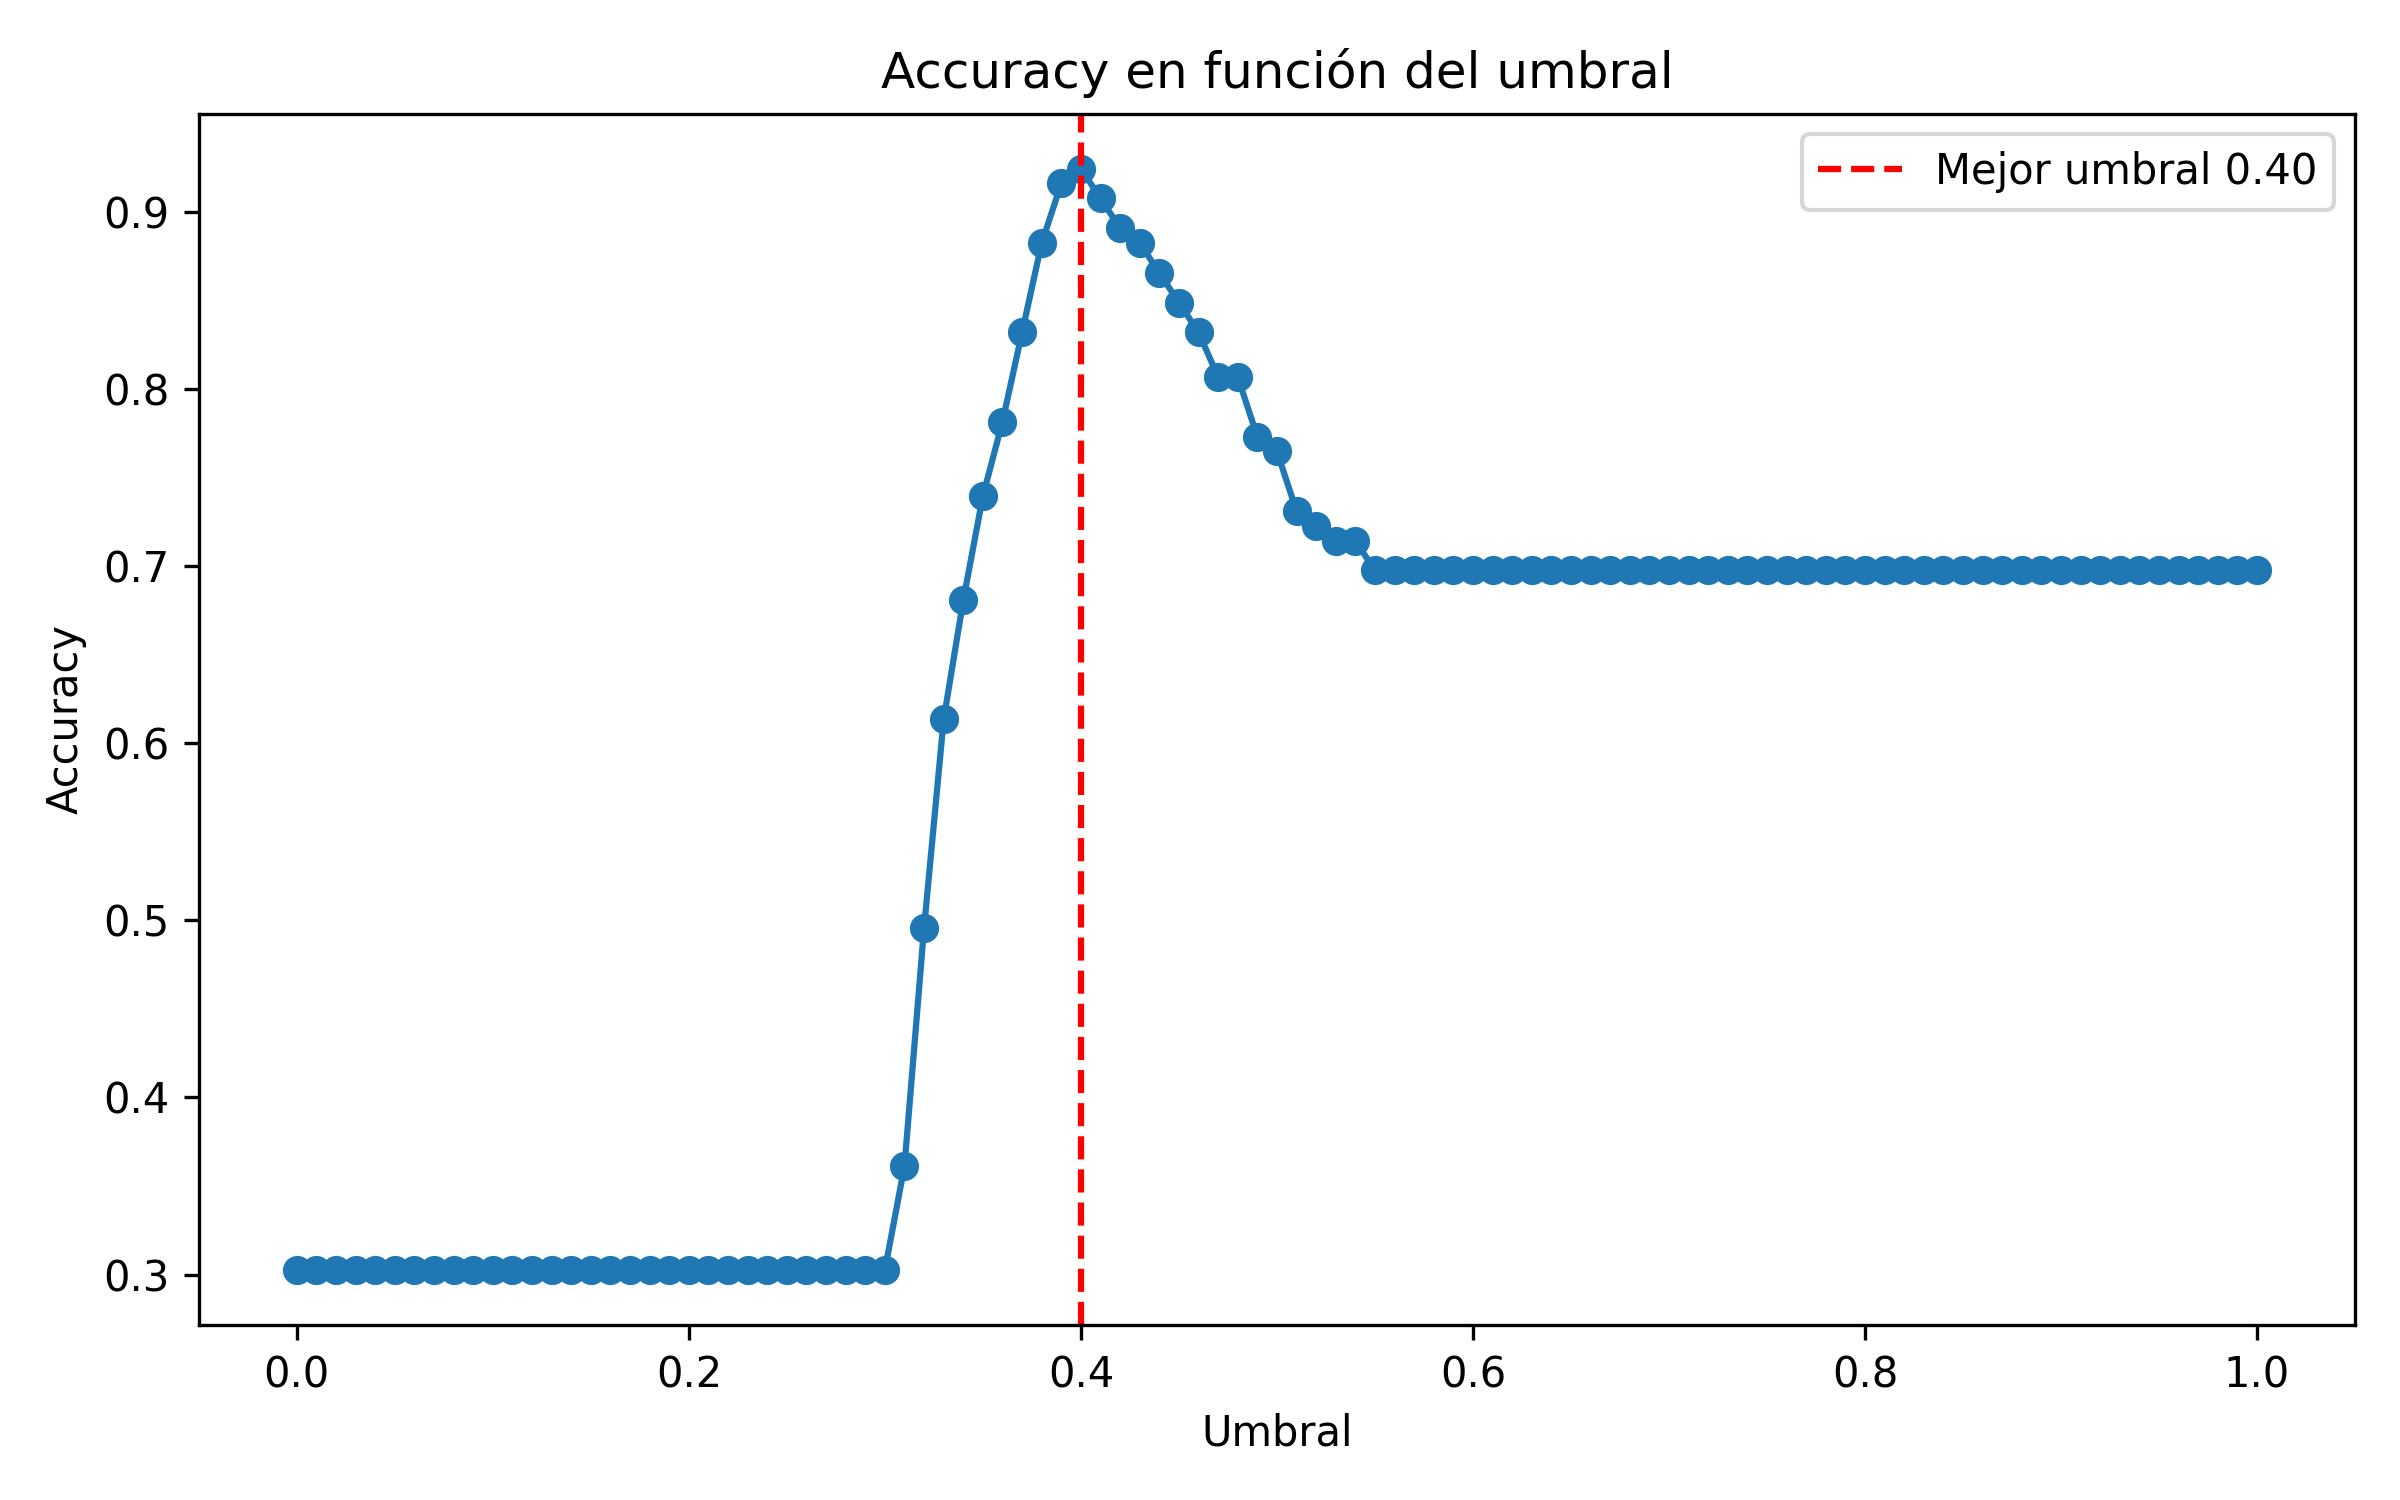
\includegraphics[width=\textwidth]{figures/accuracy_umbral.png}
			\caption{Accuracy por umbral.}
			\label{fig:accuracy-umbral}
		\end{subfigure}
		\caption{Resultados de análisis de clasificación: distribución de scores y precisión según umbral.}
		\label{fig:resultados-clasificacion}
	\end{figure}
	
	
	
	\subsection{Identificación ciencia}
	Definido el umbral se calculan estadísticos descriptivos sobre los fragmentos seleccionados.
	De los 35319 fragmentos en los que fue dividido todo el corpus de columnas, con el umbral determinado de 0.4 para la similaridad se encontraron 4287 fragmentos con menciones a la ciencia. Estos aparecen en 3004 columnas de opinión de las 13676. A nivel fragmento corresponde al 12\% y a nivel columna 22\%. 
	De esas 3004 columnas de opinión, hay un solo fragmento de ciencia en el 67.34\% (2023 columnas). Y se encuentran dos fragmentos en el 25.33\%. \\
	Esto podría ser un indicativo de que a menudo aparecen menciones a la ciencia en columnas que no tratan mayoritariamente un tema científico.
	Aunque es importante tener en cuenta que la mayoría de columnas fueron dividades en dos y tres fragmentos. 
	Se calcula que en las columnas que hay menciones de ciencia, estos fragmentos corresponden al 55.41\% del texto.
	
	\begin{figure}[H]
		\centering
		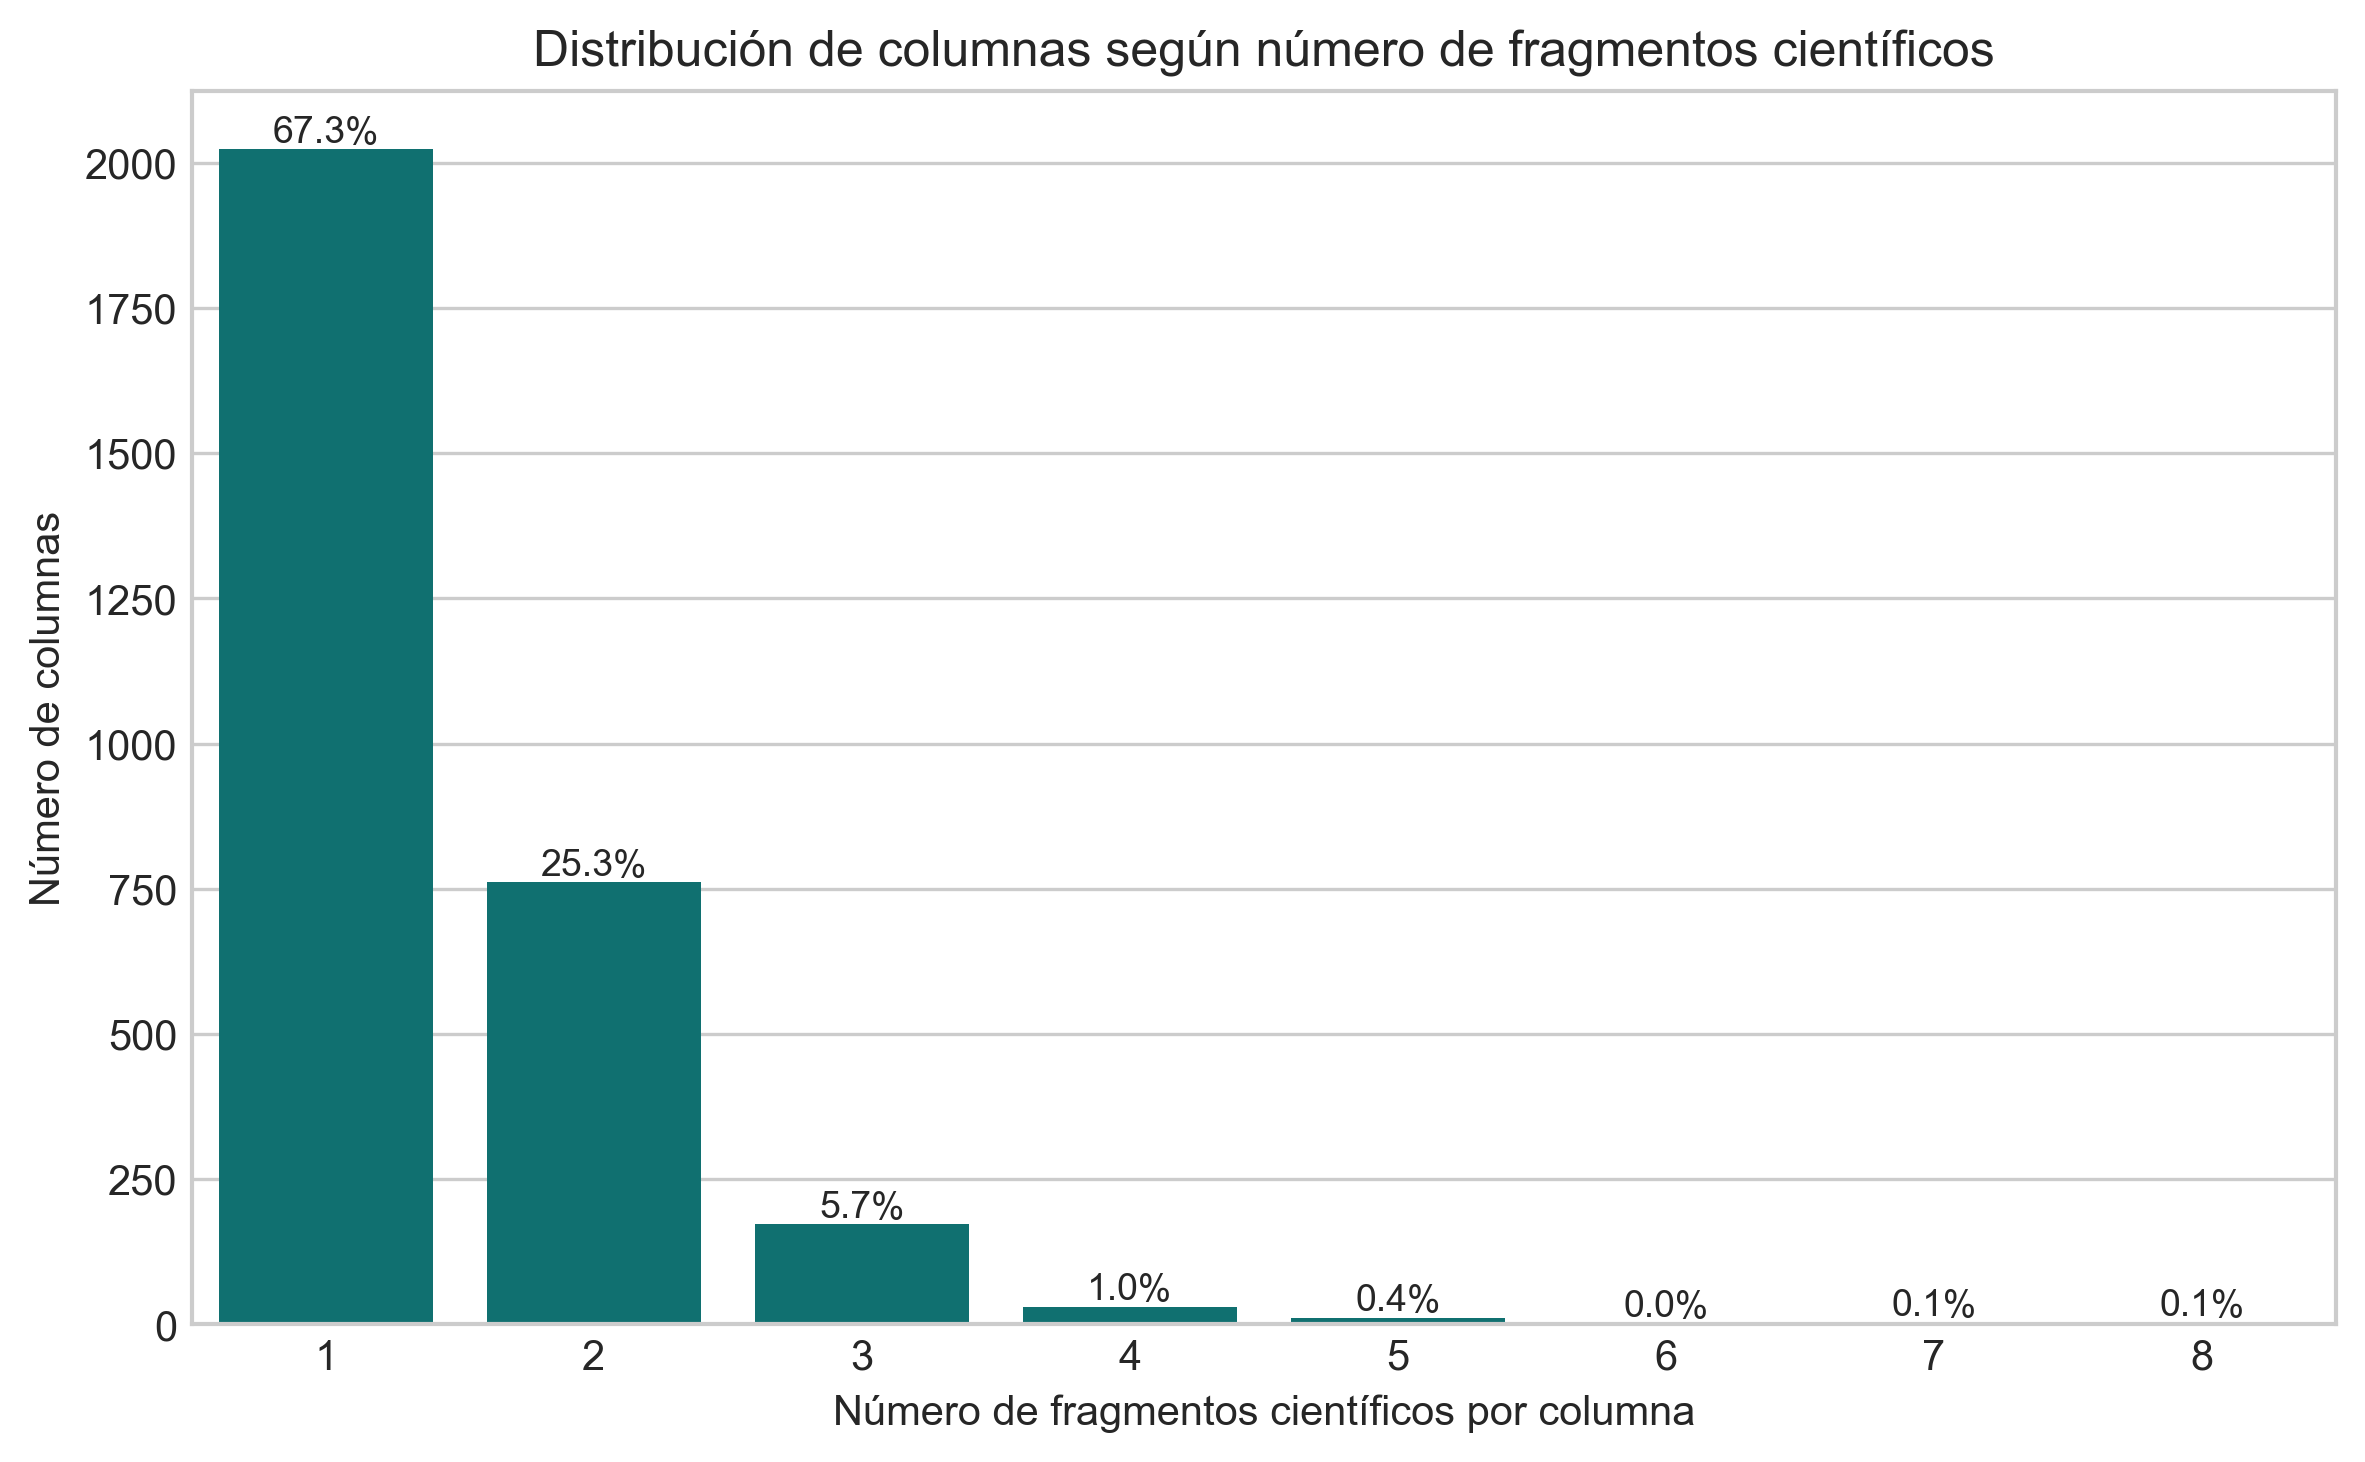
\includegraphics[width=0.9\textwidth]{figures/dist_cols_ciencia.png}
		\caption{Distribución de columnas según numero de fragmentos científicos encontrados en el texto}
		\label{fig:dist_cols_fragmentos}
	\end{figure}
	
	\subsubsection{Distribución temporal}
	La figura \ref{fig:dist_mensual_ciencia} muestra como se dan estas apariciones en toda la línea temporal. Donde más se presentan apariciones es en los meses marzo y abril del 2020, luego podemos concluir que una gran cantidad de menciones a la ciencia están relacionadas al inicio de la pandemia por el covid-19. 
	
	\begin{figure}[H]
		\centering
		
\includegraphics[width=0.95\textwidth]{figures/porcentaje_mensual_ciencia.png}
		\caption{Distribución mensual de las columnas con menciones a la ciencia}
		\label{fig:dist_mensual_ciencia}
	\end{figure}
	
	\subsubsection{Distribución por autores}
	En la Figura \ref{fig:autores_ciencia} se pueden observar los 15 autores con más menciones de ciencia en sus columnas, en dos de estos, corresponden a más del 80\% de sus columnas. Es el caso de Juan Pablo Ruiz Soto y Brigitte Baptiste. Juan Pablo Ruiz Soto fue un importante ambientalista, además economista, en el país, a menudo sus columnas de opinión trataron sobre la protección al medio ambiente.  Brigitte Baptiste es una reconocida bióloga, profesora e investigadora colombiana. 
	
	\begin{figure}[H]
		\centering
		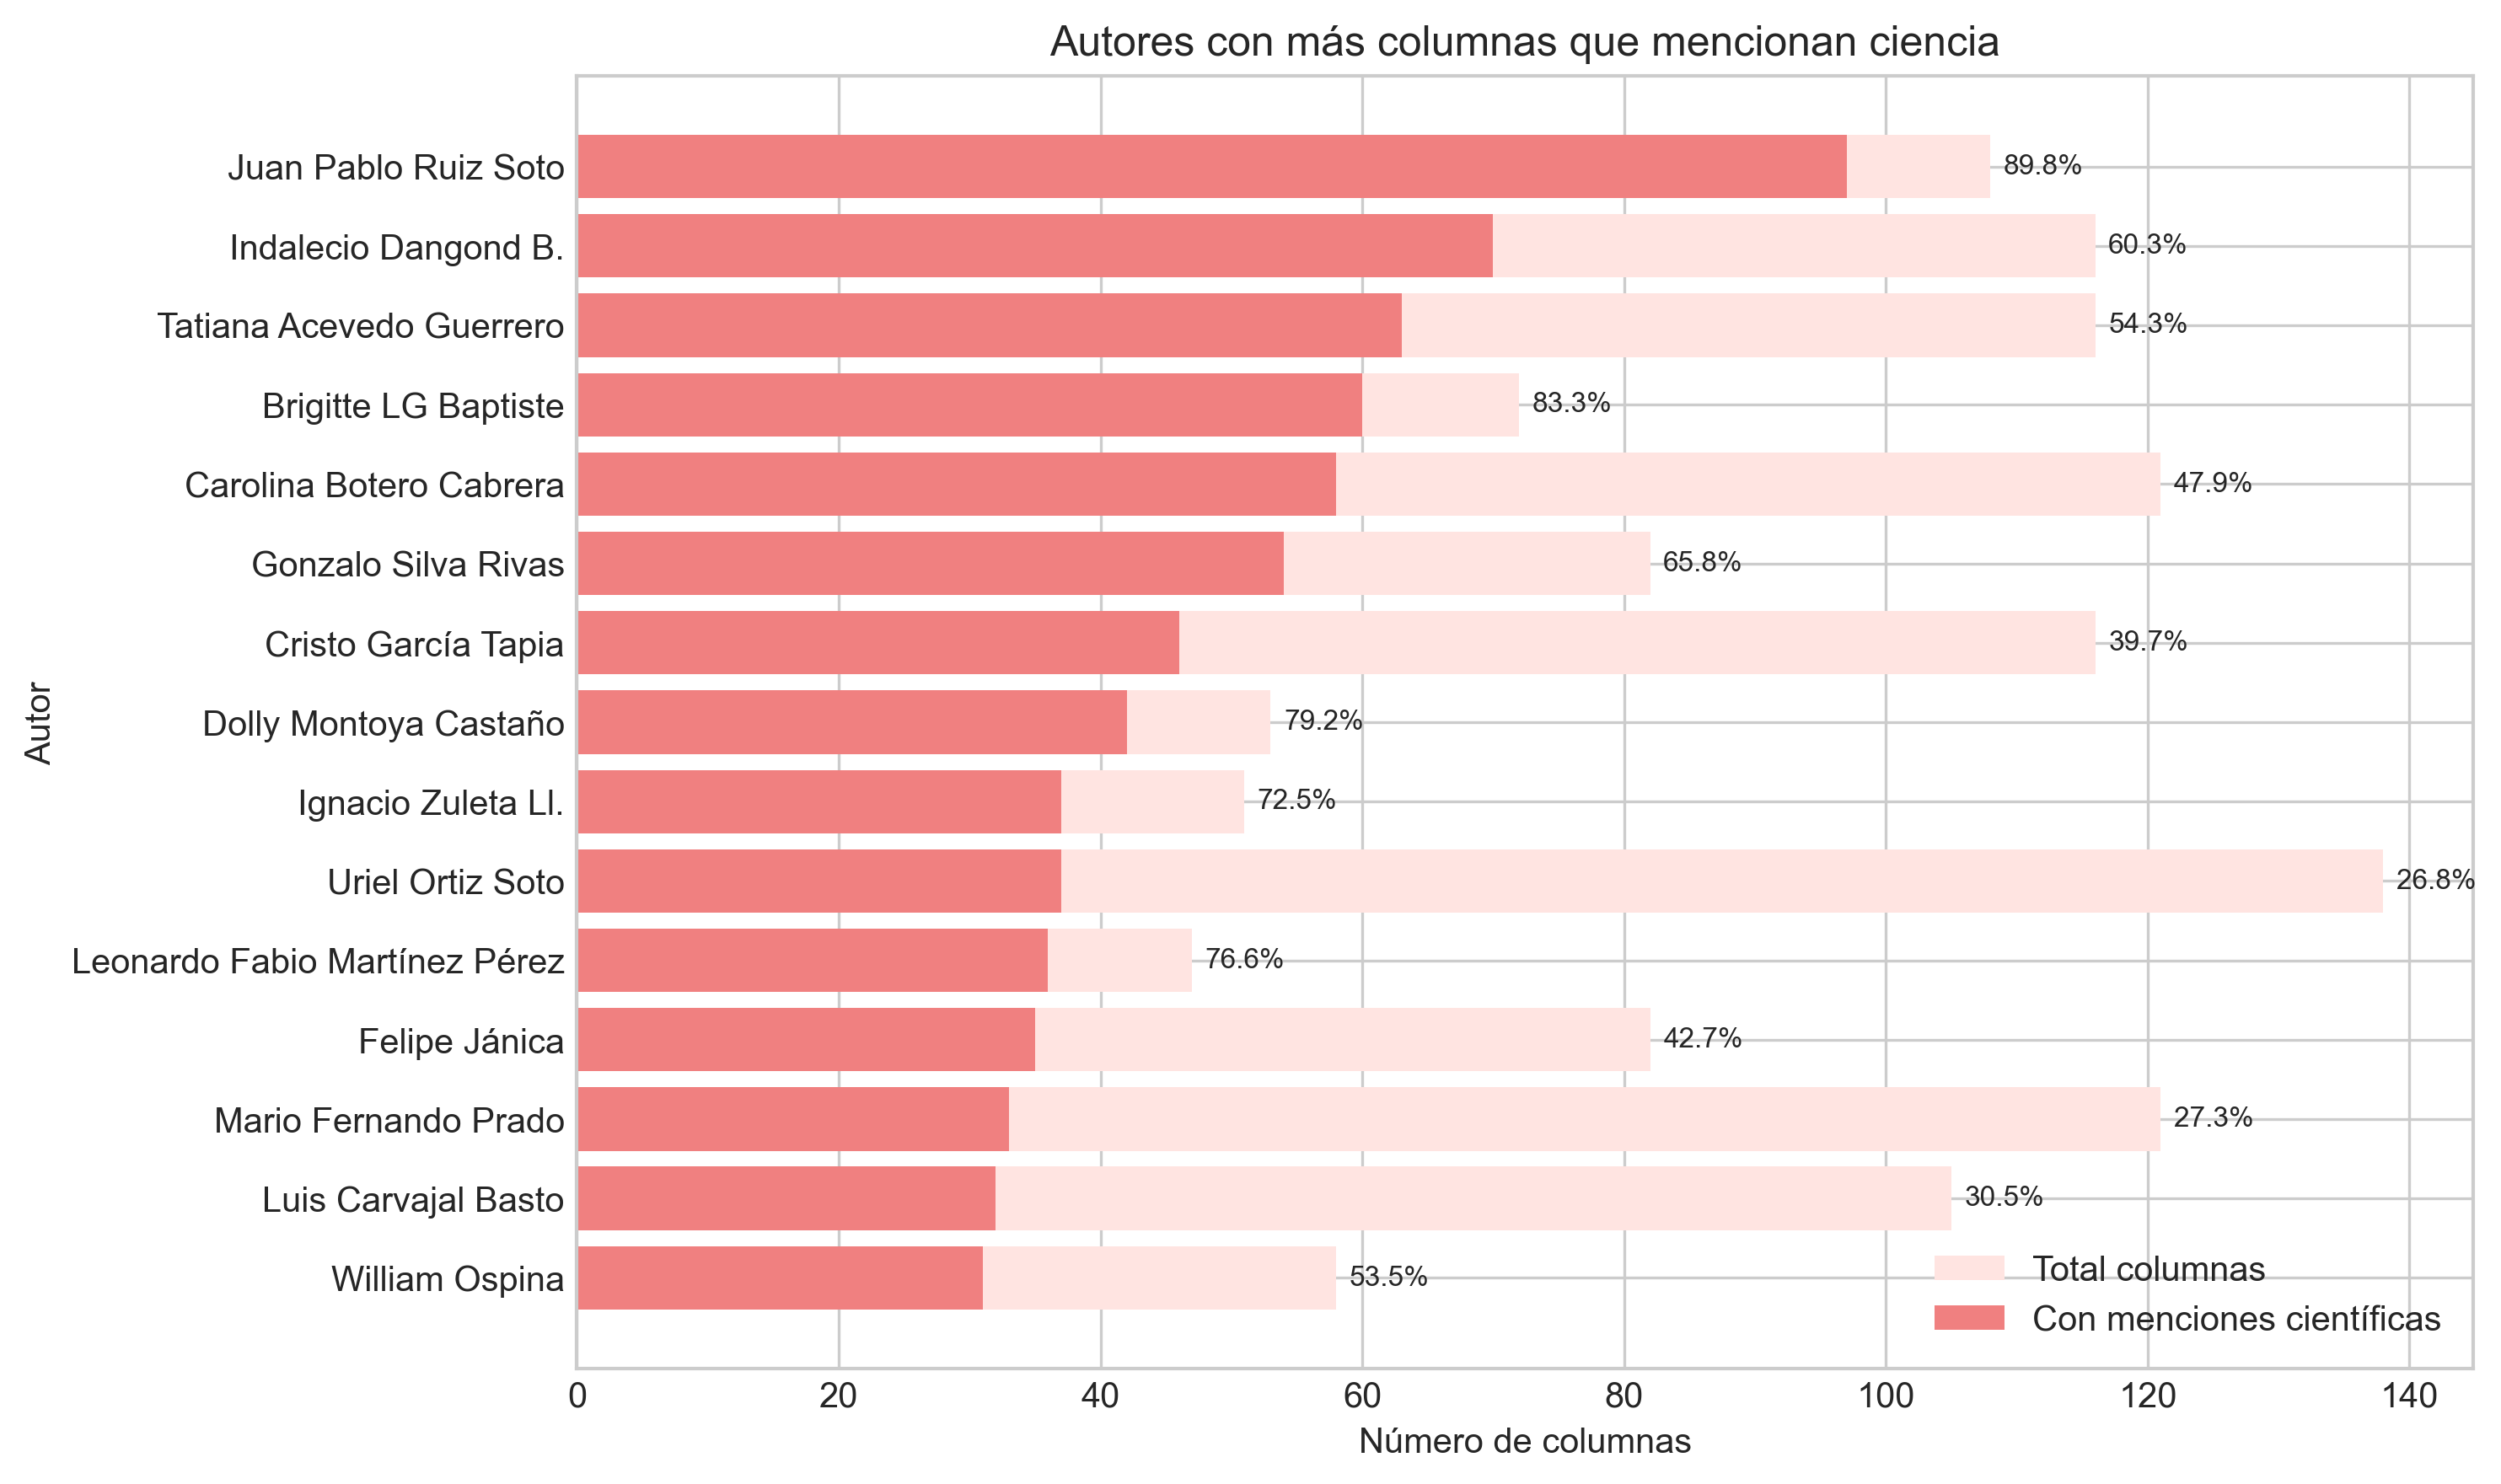
\includegraphics[width=0.95\textwidth]{figures/autores_ciencia_comparativo.png}
		\caption{Autores con más columnas con menciones de ciencia}
		\label{fig:autores_ciencia}
	\end{figure}
	
	\subsubsection{Por subcategorías}
	Cantidad de fragmentos por subcategorías. 
	\begin{figure}[H]
		\centering
		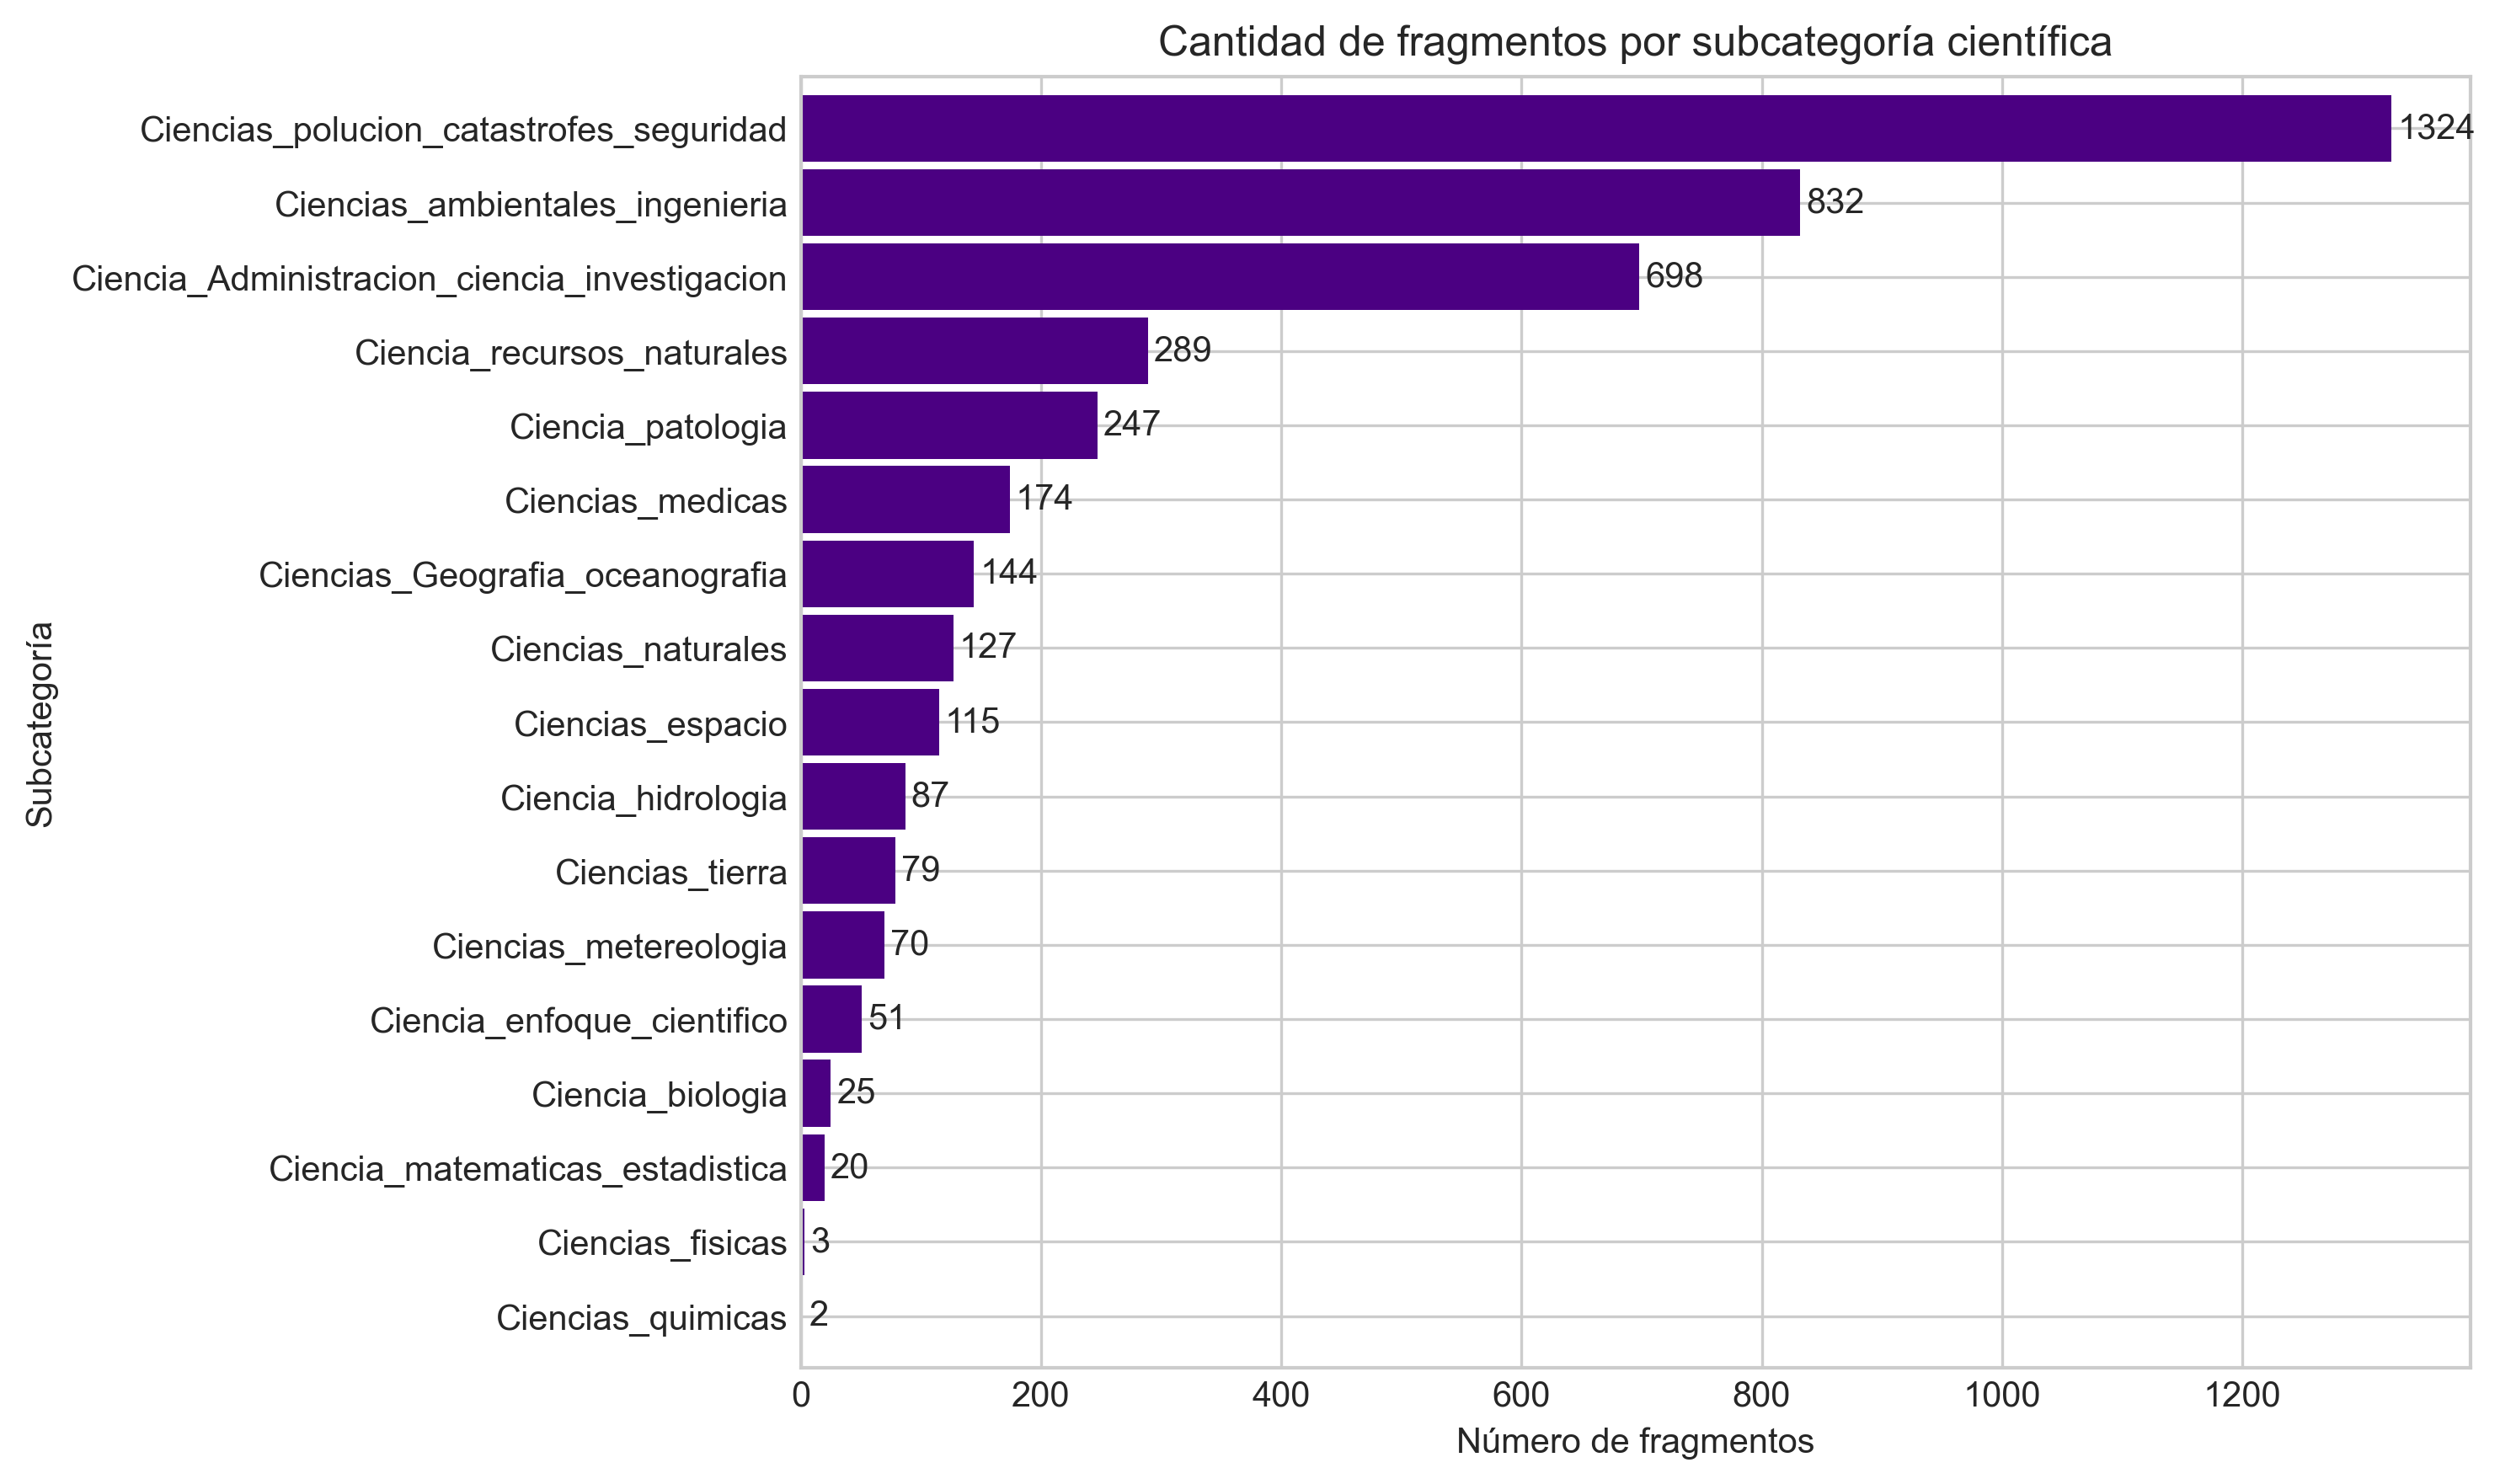
\includegraphics[width=0.95\textwidth]{figures/subcategorias_principales.png}
		\caption{Cantidad de fragmentos por subcategoría}
		\label{fig:subcat_fragmentos}
	\end{figure}
	Esto nos habla de que cuando se habla de ciencia en estas columnas de opinión principalmente se hace desde cuestiones medio ambientales y de como se administra la ciencia en el país y no tanto desde lo físico o lo químico.
	
	INCLUIR EJEMPLOS
	
	\subsubsection{Nubes de palabras}
	\begin{figure}[H]
		\centering
		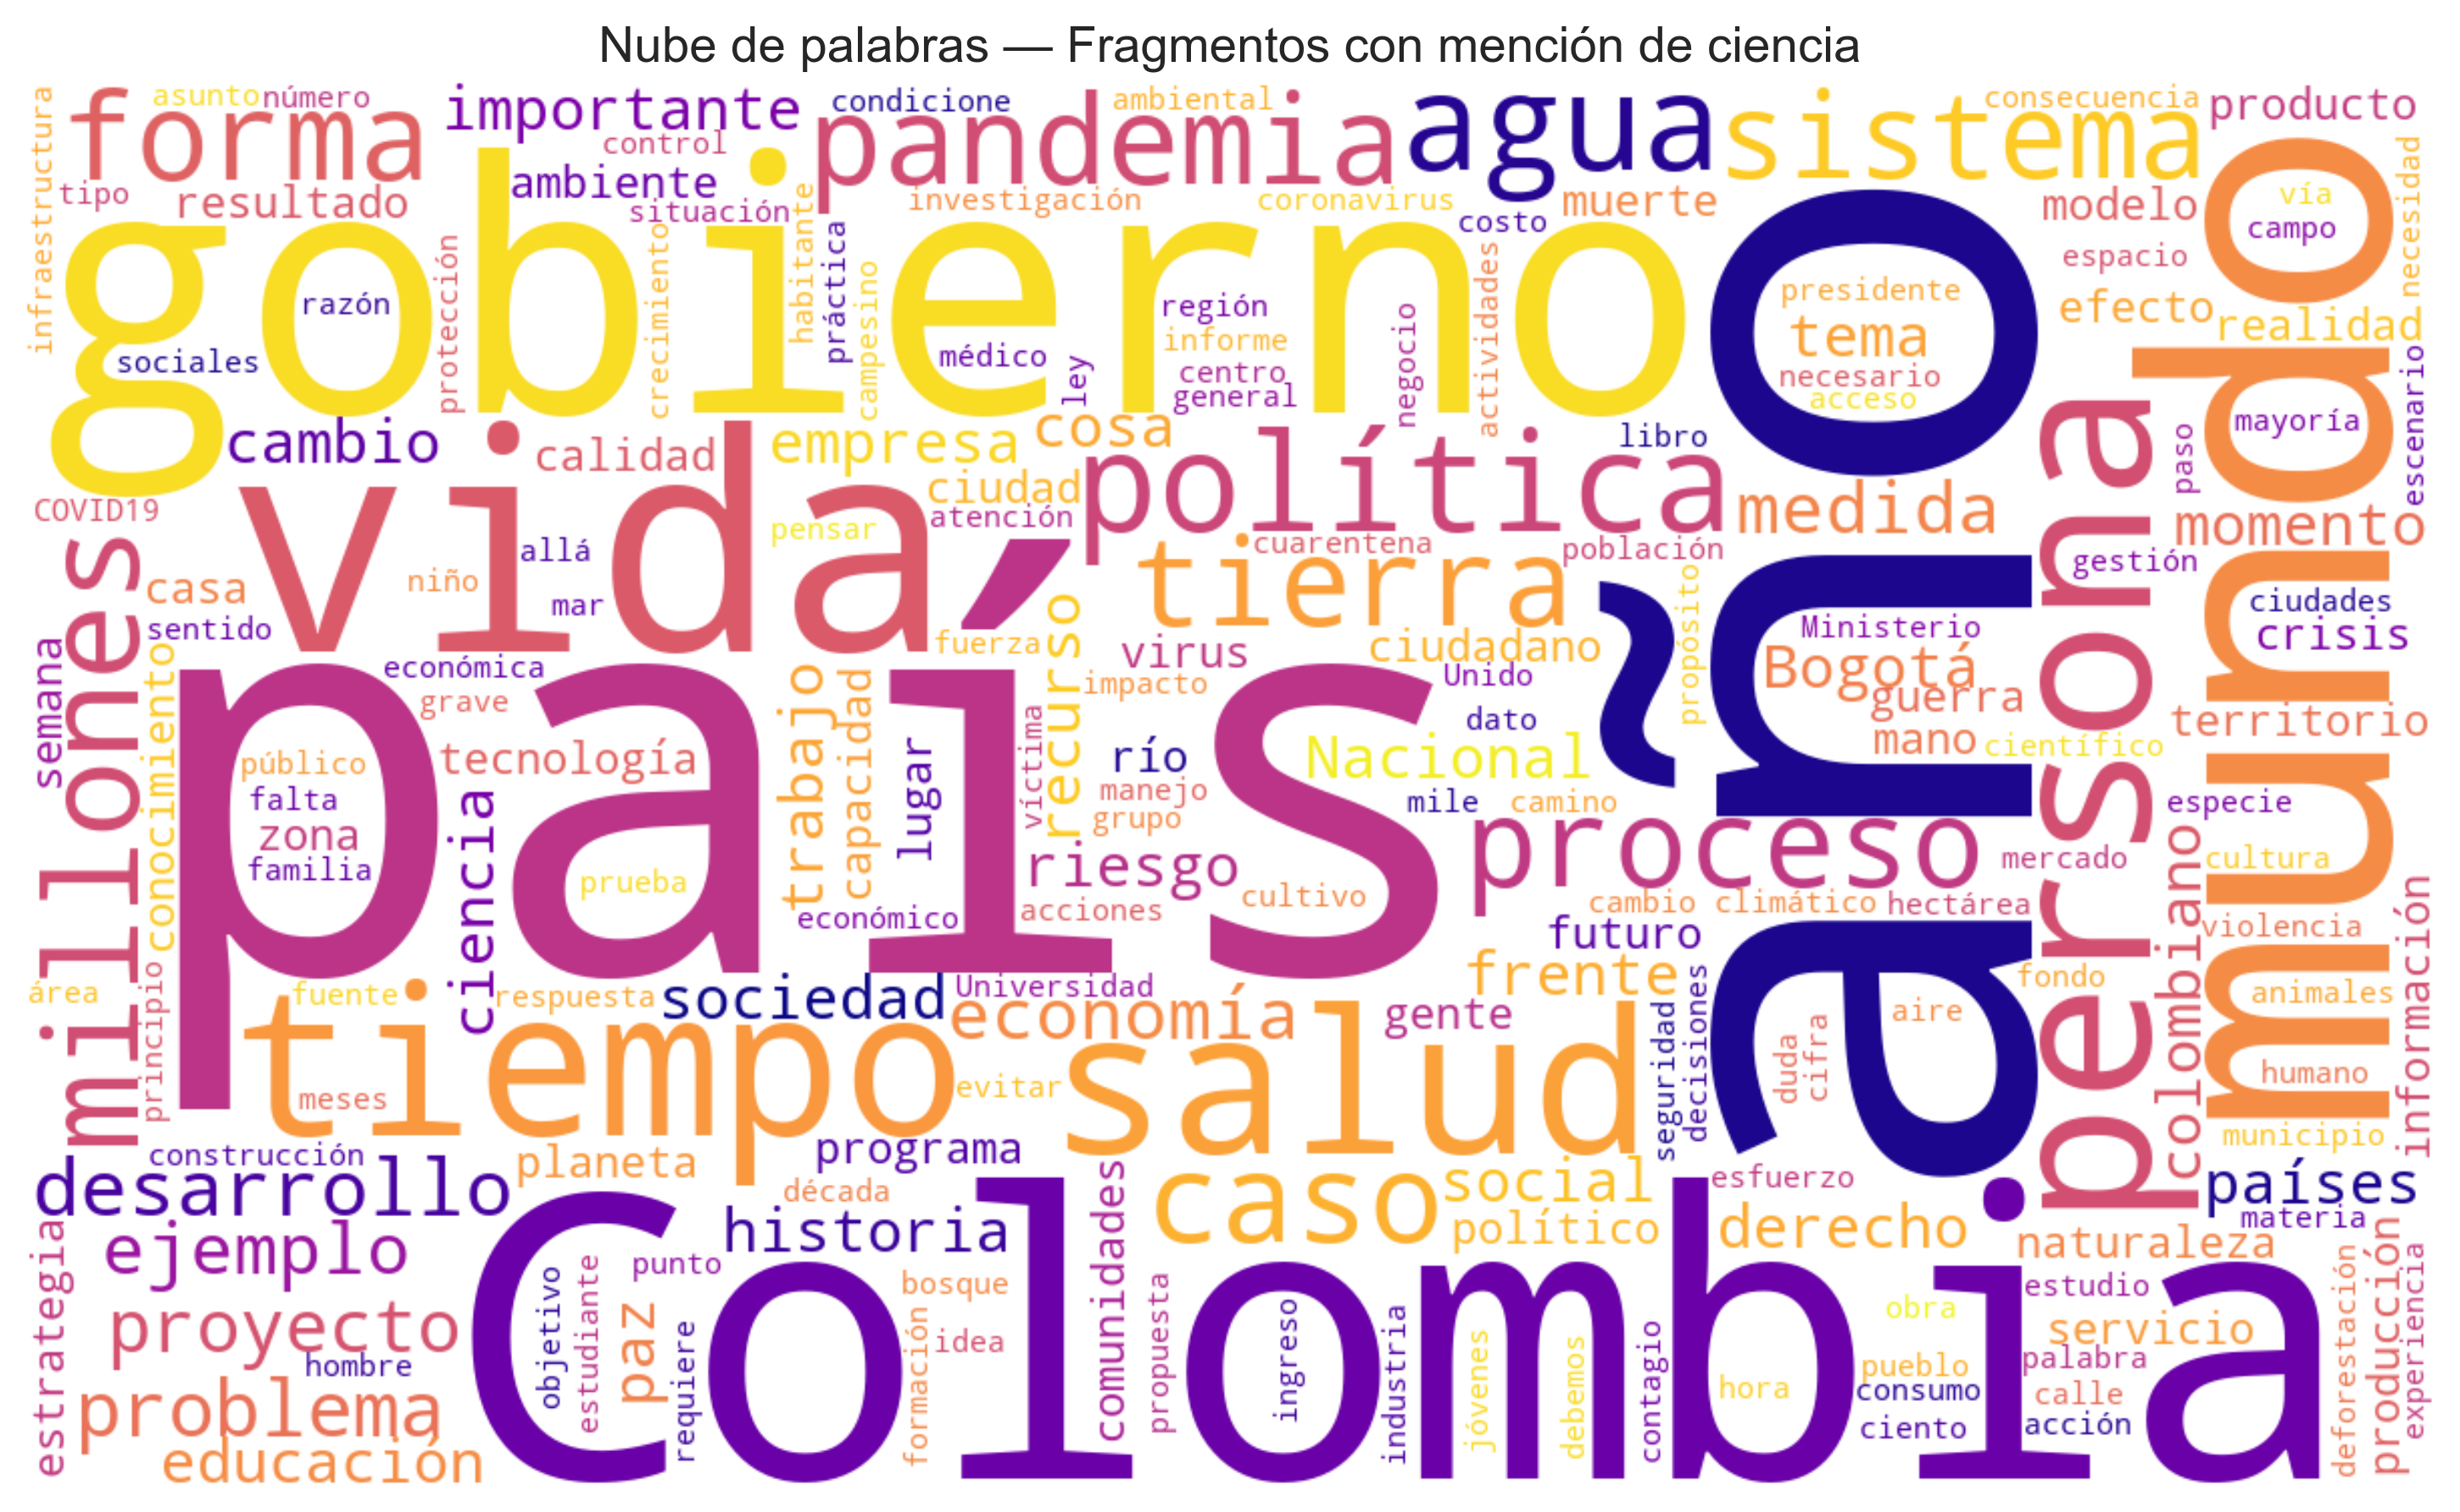
\includegraphics[width=0.95\textwidth]{figures/nube_ciencia_fragmentos.png}
		\caption{Nube de palabras de los fragmentos seleccionados}
		\label{fig:frag_ciencia}
	\end{figure}
	
	
	\subsection{Análisis por palabras}
	
	Esta tabla incluye las palabras más frecuentes en las columnas con al menos una mención de ciencia. Estas columnas representan el 22\% del corpus, luego es interesante observar que palabras aparecen en las columnas con menciones de ciencia en proporción mayor a este número. El 50\% de apariciones de la palabra salud aparece relacionada a ciencia. Asi tambien el 62\% de apariciones de agua, el 51\% de pandemia, 45\% desarrollo 41\% recursos, 40\% universidad. Esto indica que a menudo las menciones de ciencia son las que capturan la mayor parte de la presencia de términos relacionados con la pandemia y la salud, también con el desarrollo, agua y recursos (medio ambiente), también universidad (educación).
	
	\begin{table}
		\begin{center}
			\begin{table}[H]
\caption{Palabras más frecuentes en columnas con mención científica respecto al corpus.}
\label{tab:frecuencias_columnas}
\begin{tabular}{lrrr}
\toprule
Palabra & Freq. corpus & Freq. columnas ciencia & Proporción columnas \\
\midrule
país & 16307 & 3734 & 0.23 \\
colombia & 14604 & 3302 & 0.23 \\
nacional & 7499 & 2418 & 0.32 \\
años & 13137 & 2855 & 0.22 \\
mundo & 8676 & 2533 & 0.29 \\
gobierno & 14310 & 2757 & 0.19 \\
salud & 3958 & 1924 & 0.49 \\
vida & 8455 & 2248 & 0.27 \\
desarrollo & 3621 & 1629 & 0.45 \\
millones & 5939 & 1717 & 0.29 \\
personas & 6180 & 1695 & 0.27 \\
agua & 1888 & 1177 & 0.62 \\
social & 5459 & 1599 & 0.29 \\
tiempo & 6547 & 1670 & 0.26 \\
política & 9897 & 1753 & 0.18 \\
pandemia & 2510 & 1276 & 0.51 \\
recursos & 2988 & 1236 & 0.41 \\
año & 5760 & 1514 & 0.26 \\
educación & 3924 & 1322 & 0.34 \\
sistema & 3960 & 1183 & 0.30 \\
cambio & 4241 & 1120 & 0.26 \\
países & 4462 & 1185 & 0.27 \\
economía & 4114 & 1181 & 0.29 \\
sociedad & 4542 & 1152 & 0.25 \\
sociales & 4639 & 1184 & 0.26 \\
universidad & 2813 & 1117 & 0.40 \\
forma & 4185 & 1103 & 0.26 \\
crisis & 3094 & 1063 & 0.34 \\
paz & 8114 & 1282 & 0.16 \\
ejemplo & 4244 & 1049 & 0.25 \\
\bottomrule
\end{tabular}
\end{table}

		\end{center}
	\end{table}
	
	\subsection{Coocurrencias}
	
	\subsection{Entidades reconocidas}
	
	\begin{figure}[H]
		\centering
		\begin{subfigure}[t]{0.32\textwidth}
			\centering
			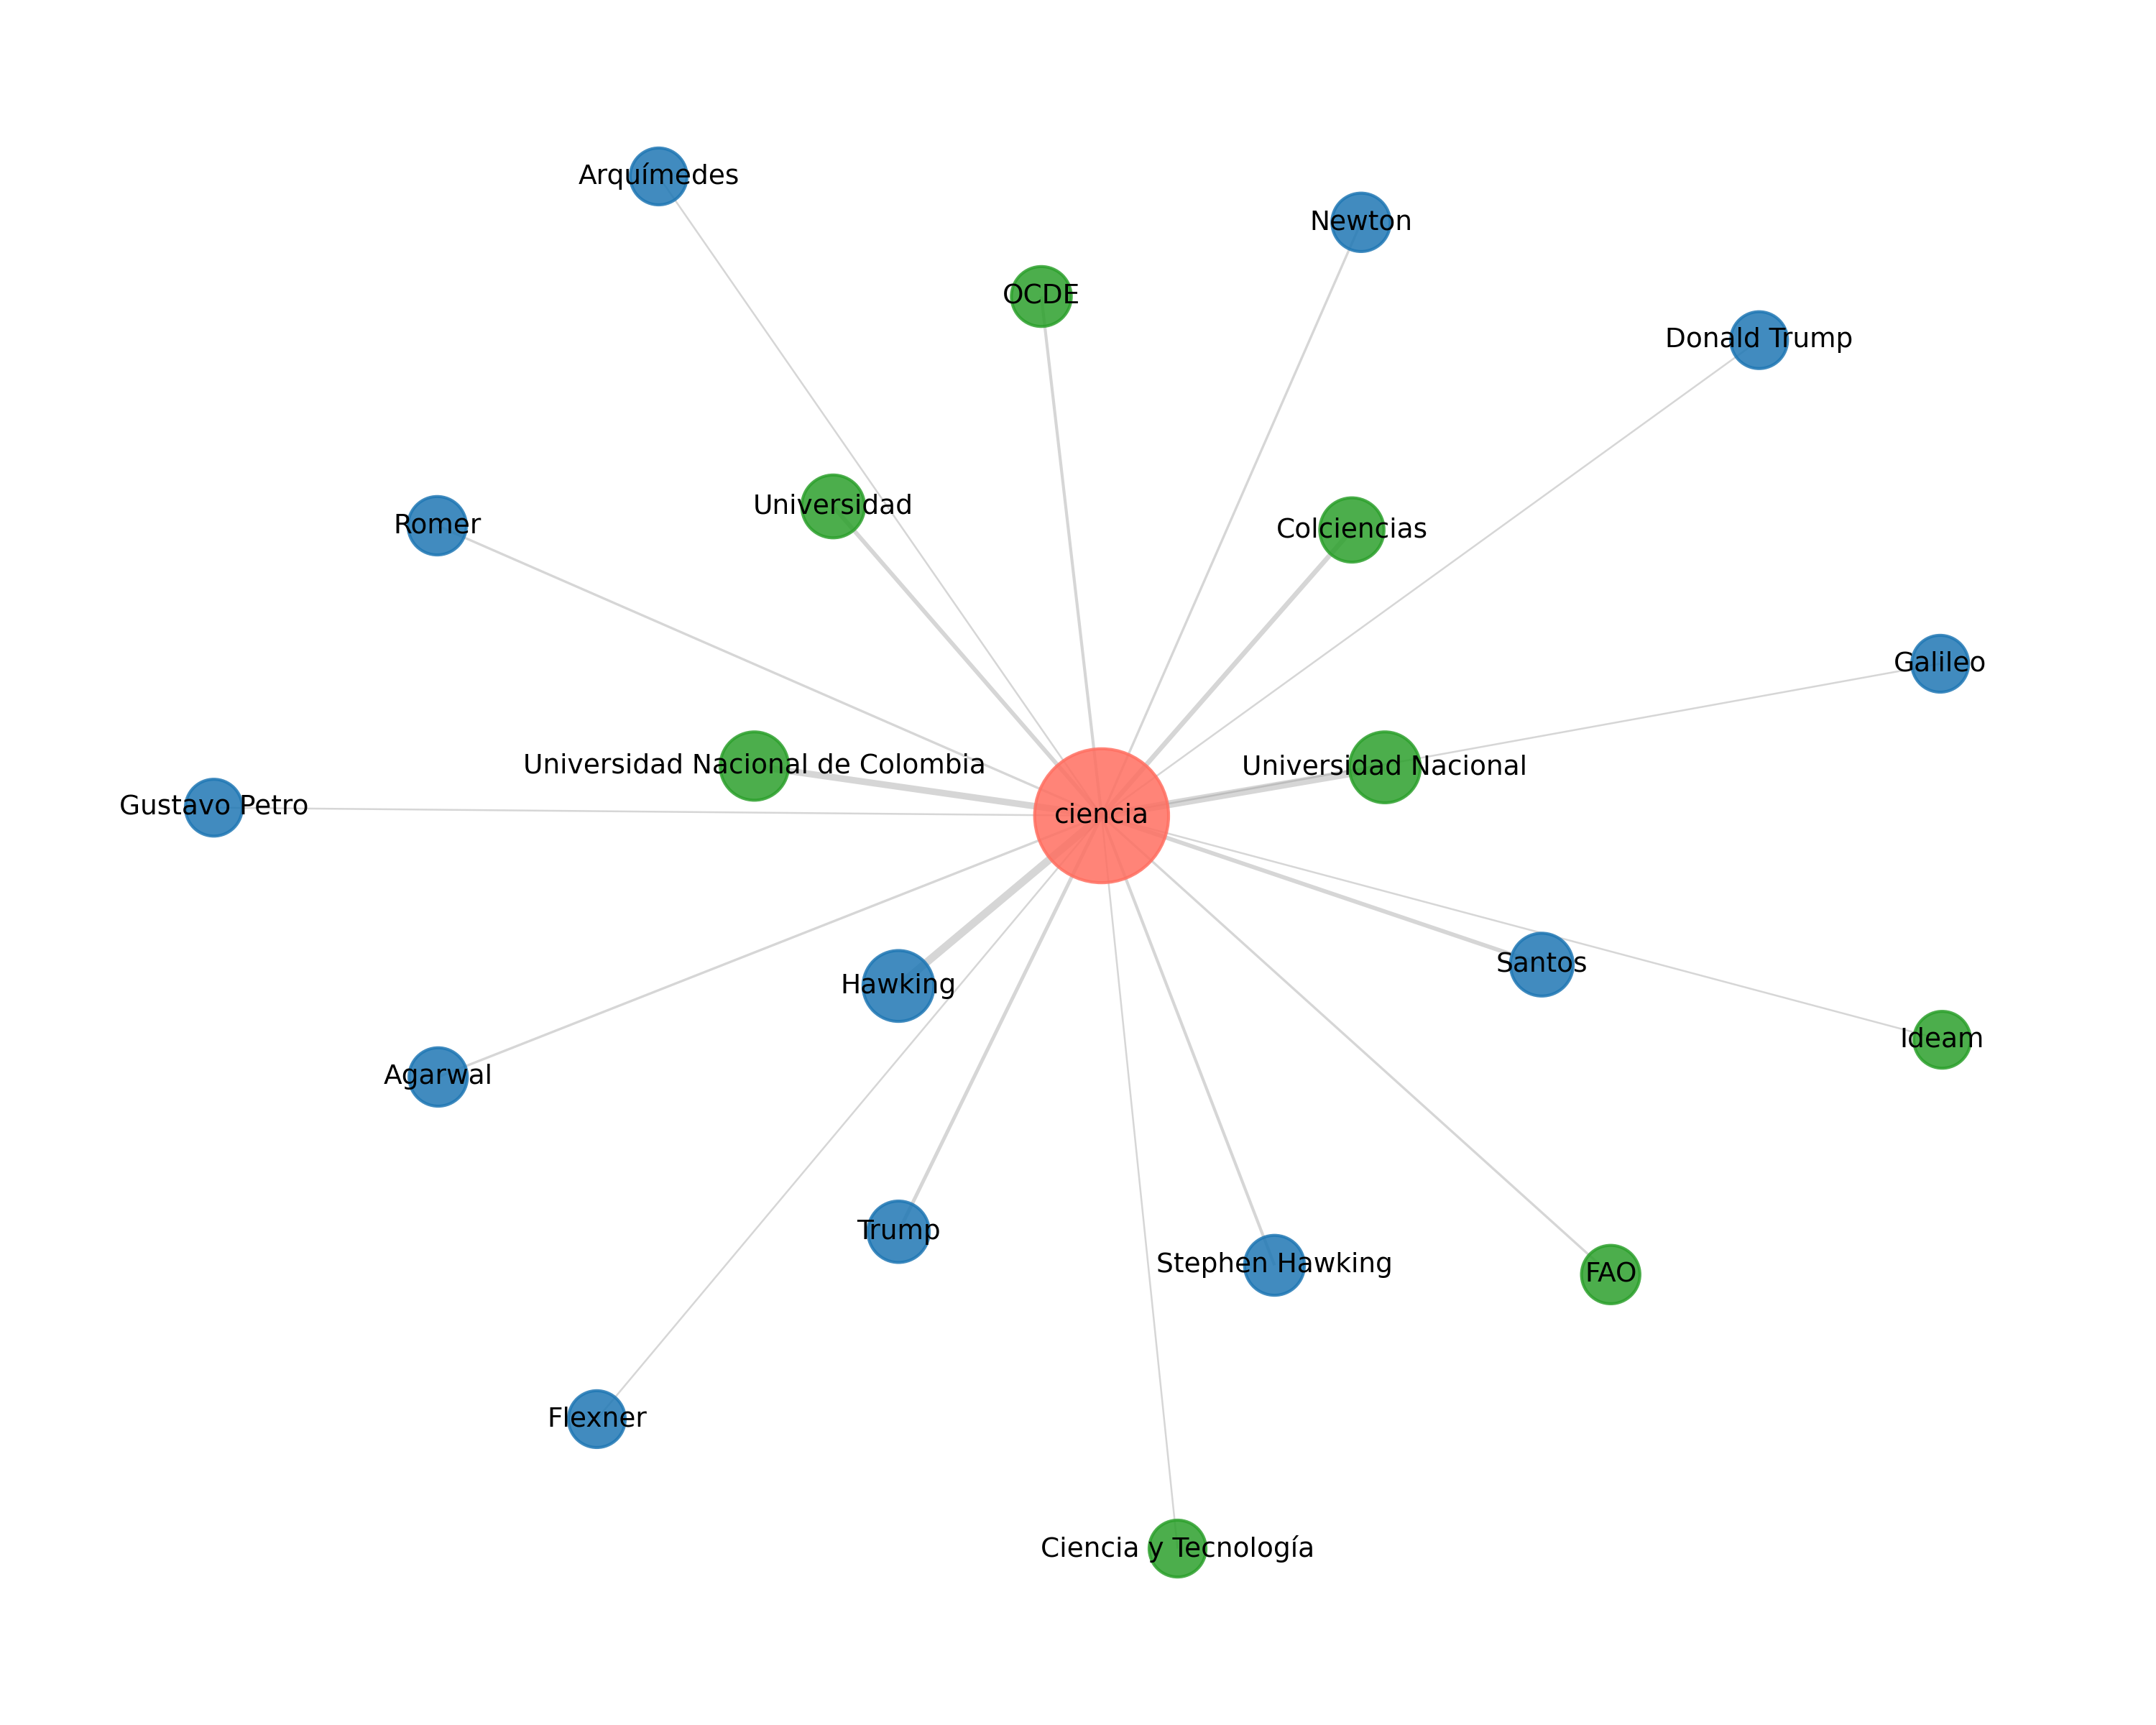
\includegraphics[width=\textwidth]{figures/grafo_ciencia_2018.png}
			\caption{2018}
			\label{fig:grafo_ciencia_2018}
		\end{subfigure}
		\hfill
		\begin{subfigure}[t]{0.32\textwidth}
			\centering
			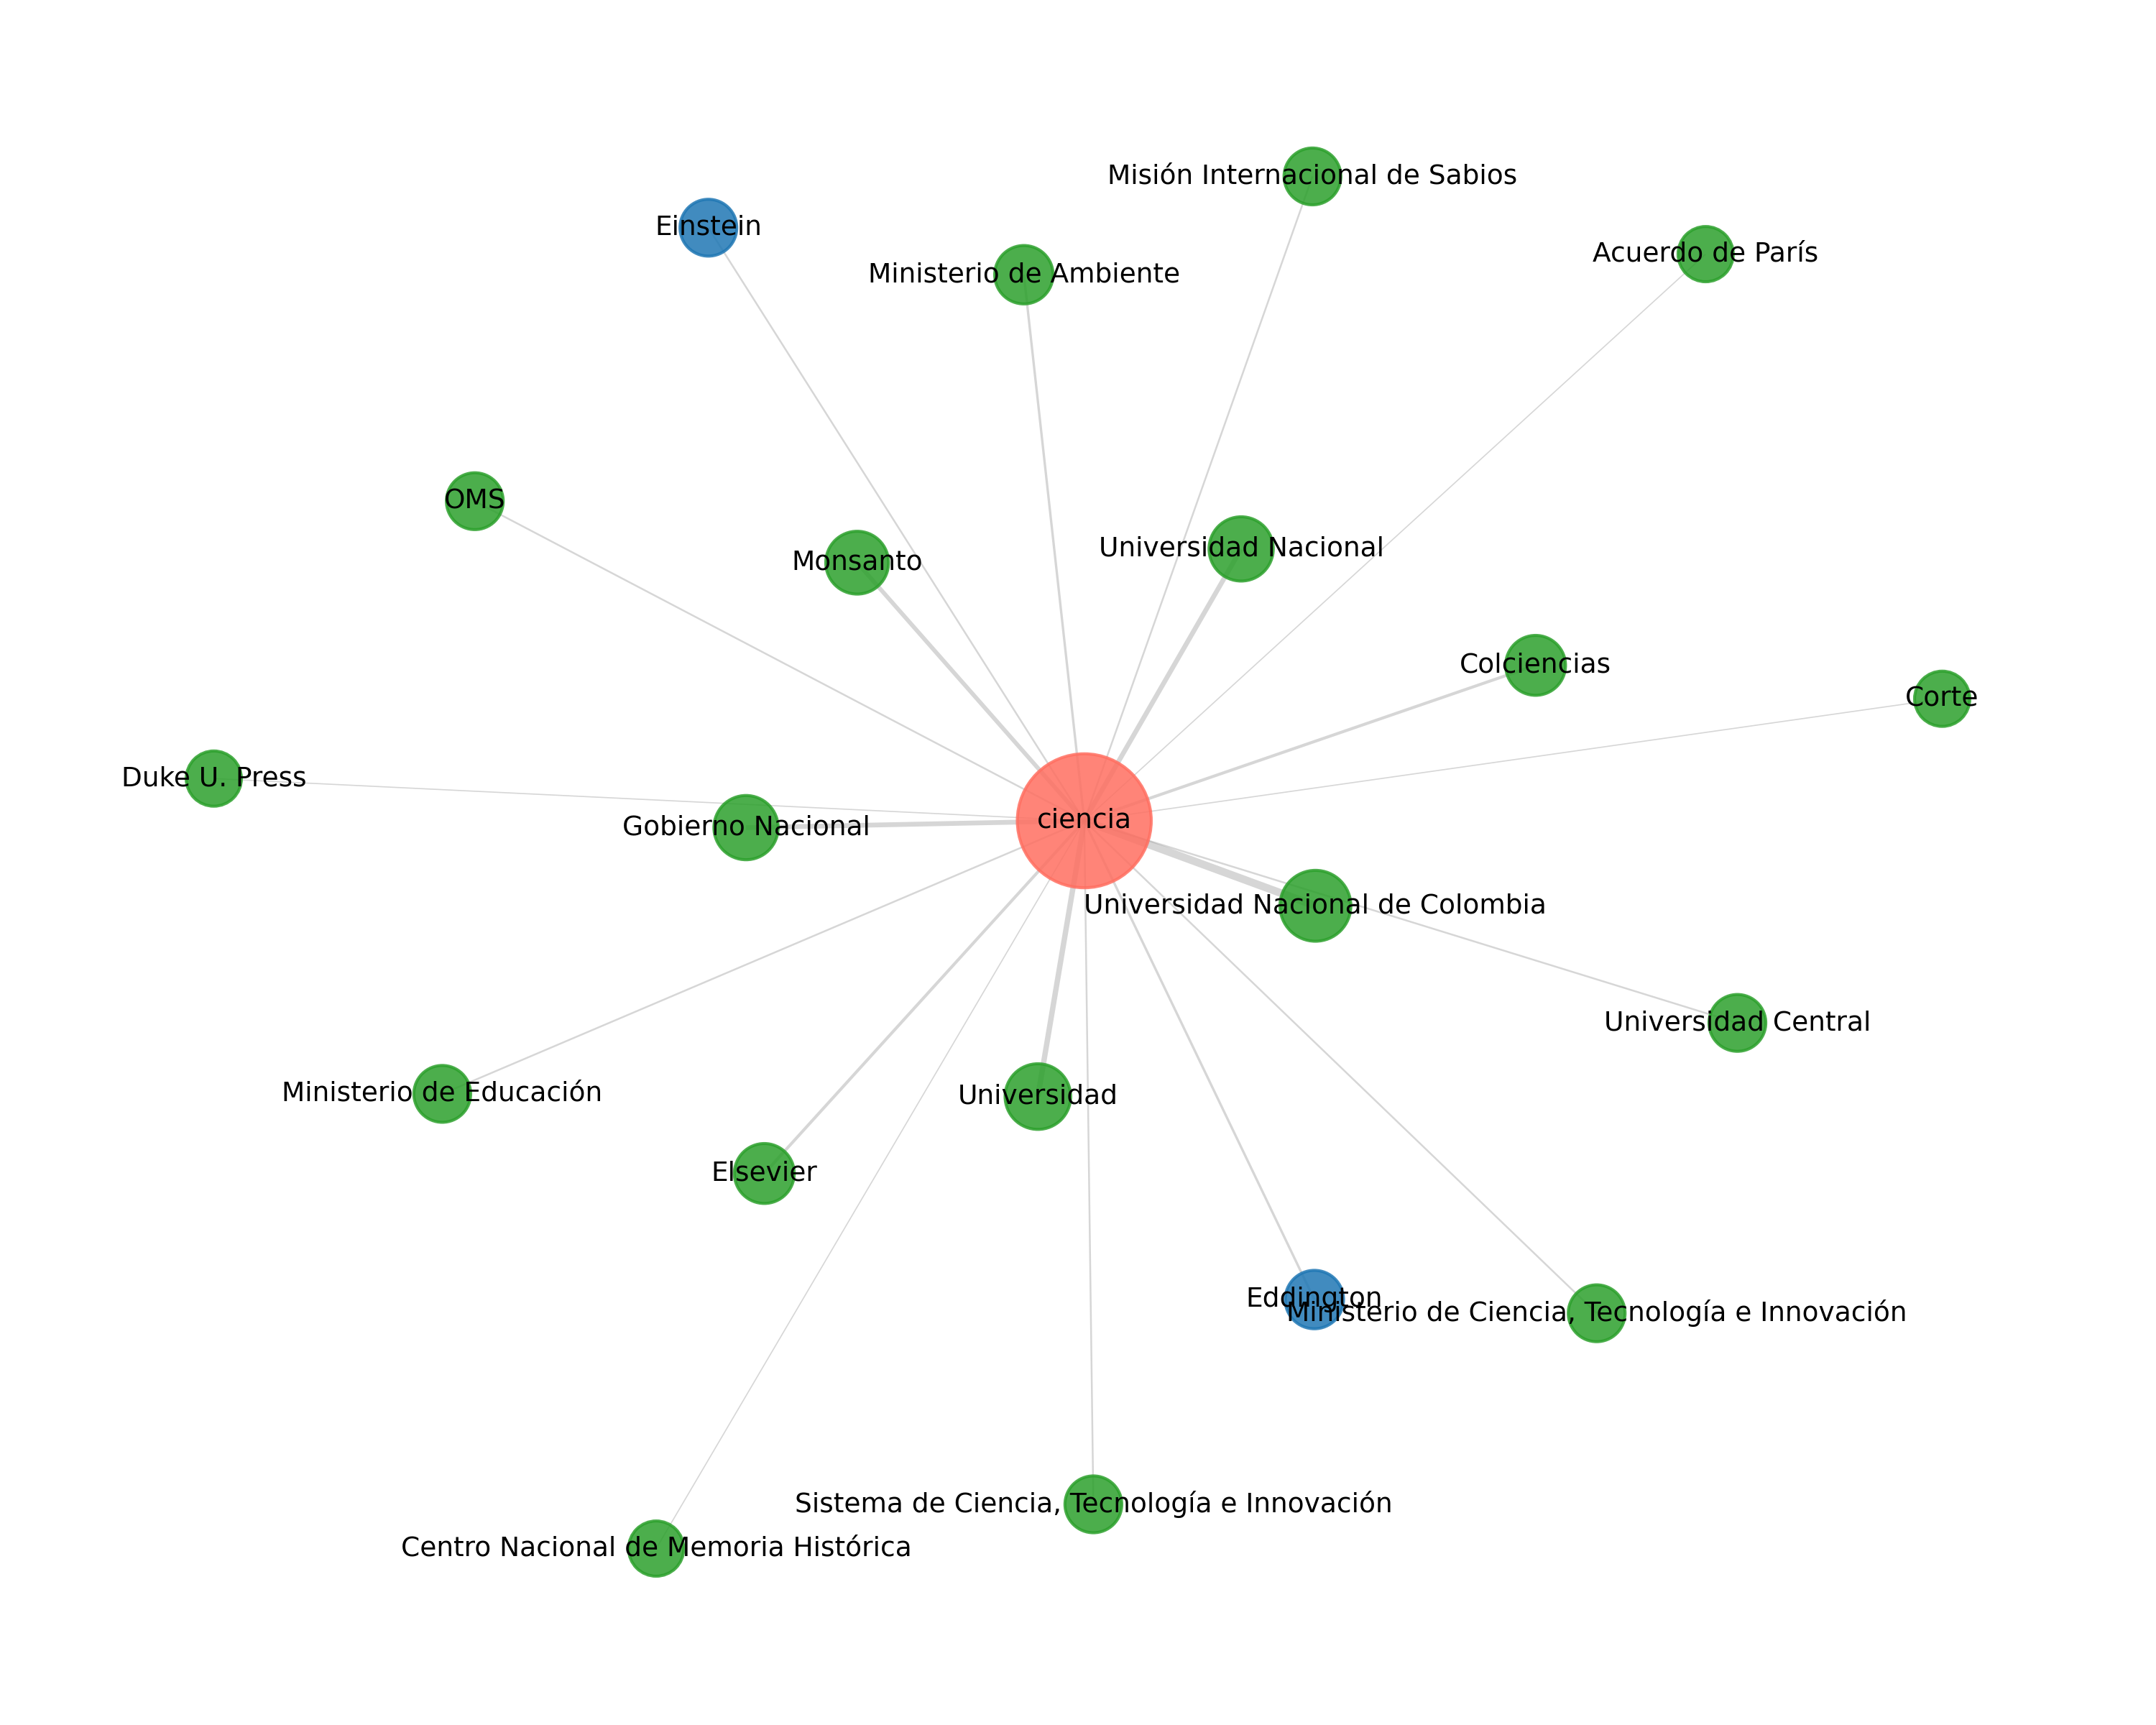
\includegraphics[width=\textwidth]{figures/grafo_ciencia_2019.png}
			\caption{2019}
			\label{fig:grafo_ciencia_2019}
		\end{subfigure}
		\hfill
		\begin{subfigure}[t]{0.32\textwidth}
			\centering
			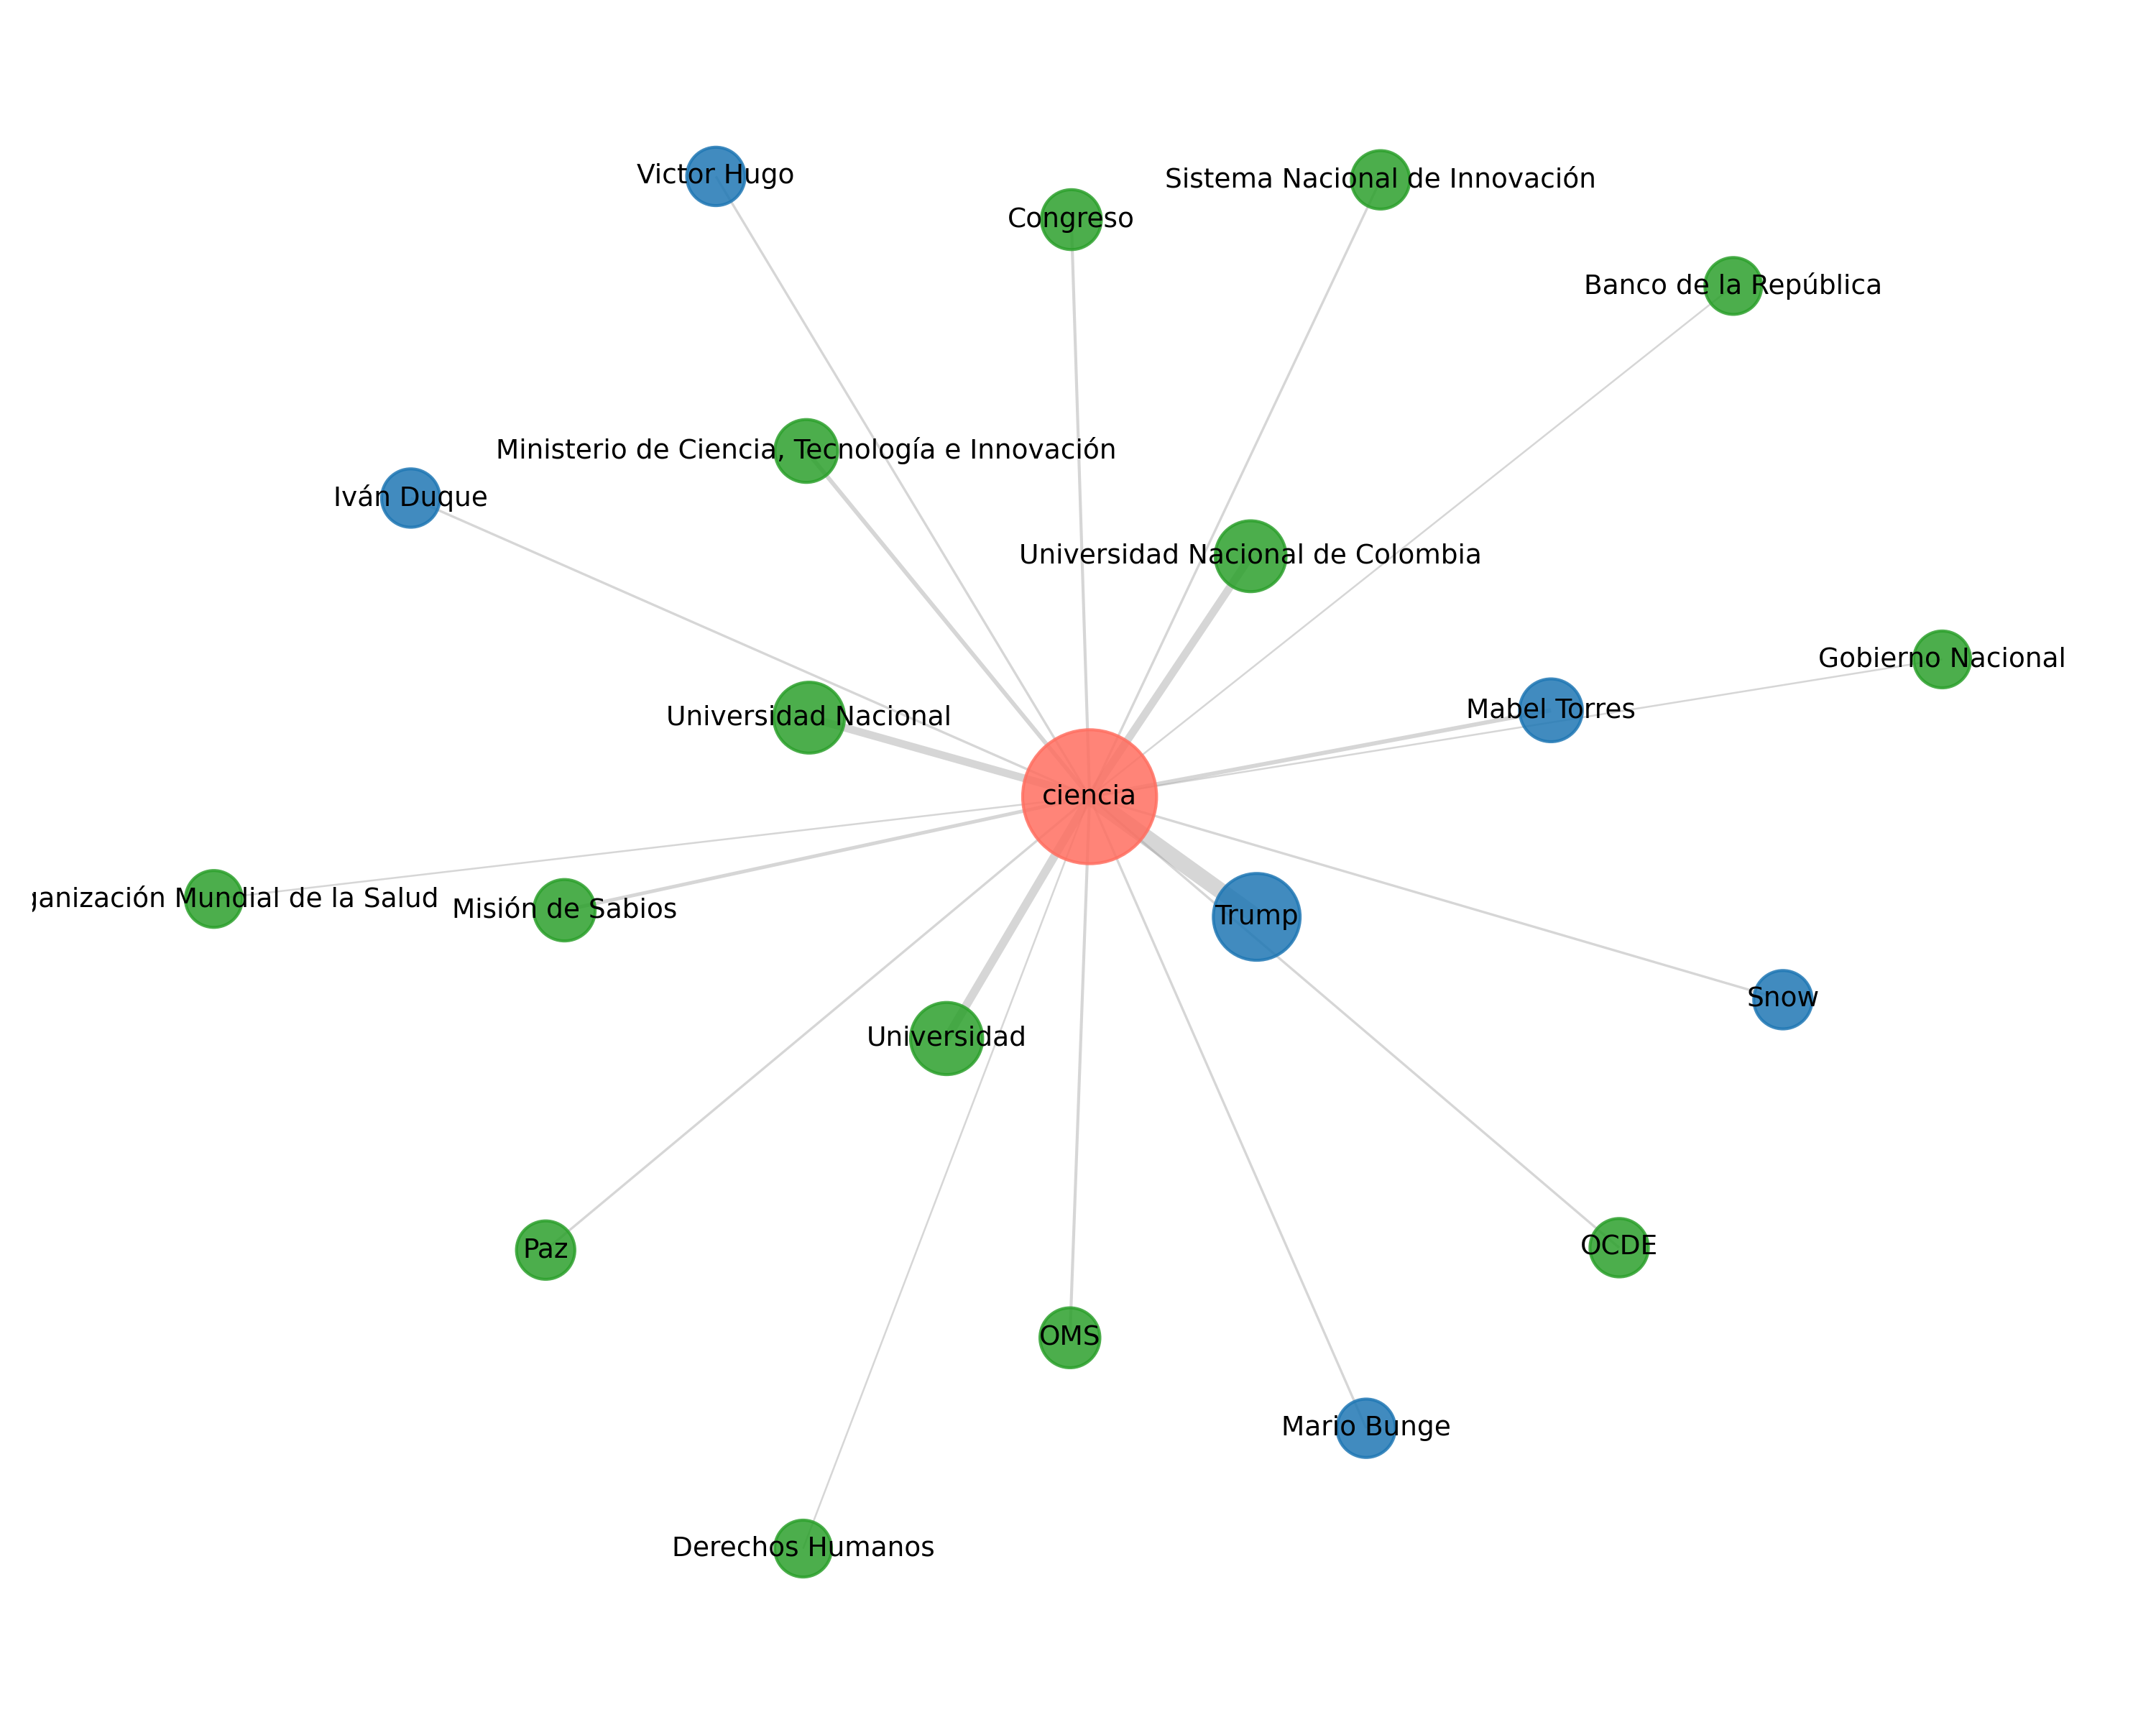
\includegraphics[width=\textwidth]{figures/grafo_ciencia_2020.png}
			\caption{2020}
			\label{fig:grafo_ciencia_2020}
		\end{subfigure}
		\caption{Redes de entidades (personas y organizaciones) asociadas al término \textit{ciencia} en columnas de opinión, por año.}
		\label{fig:grafos_ciencia_anuales}
	\end{figure}
	
	
	Tengo una lista de entidades ya. Decidir como mostrar alguna cosa de ahí.
	Algunas organizaciones interesantes:
	Universidades, ONU, Universidad Nacional de Colombia
	Unión Europea
	Universidad Pedagógica Nacional
	OMS
	OCDE
	UCI
	Ministerio de Ambiente
	Ministerio de Agricultura
	Google
	Colciencias
	Ministerio de Educación
	ICA
	Amazon
	Ministerio de Educación Nacional
	Netflix
	Unesco
	Ministerio de Ciencia, Tecnología e Innovación
	Ministerio del Interior
	NASA
	Sena
	Universidad de Harvard
	Academia Nacional de Medicina
	Harvard
	IPCC
	Instituto Nacional de Salud
	Karisma
	Microsoft
	Agencia Internacional para la Investigación del Cáncer
	Agencia Nacional de Licencias Ambientales
	Alianza Colombia Libre de Fracking
	Otras 66 nombres de universidades que salen solo una vez
	
	
	Algunas personas, además de muchos politicos:
	Stephen Hawking
	Humboldt
	papa Francisco
	Buda
	Greta Thunberg
	Newton
	Camus
	Darwin
	Brigitte Baptiste

	
	
	
	
	
	
	Resumen de hallazgos cuantitativos (frecuencias, tópicos, marcos) y cualitativos (funciones argumentativas, retóricas, simbólicas). 


	
	\section{Discusión}
	Posibles temas a discutir (IA)
	\begin{itemize}
		\item La ciencia aparece asociada principalmente a temas políticos e institucionales, no a temas estrictamente científicos.
		\item La ciencia aparece en la esfera pública sobre todo en relación con crisis o eventos coyunturales (pandemia, corrupción, debates regulatorios).
		\item La ciencia es mayormente representada en marcos discursivos de riesgo y controversia más que en marcos de innovación o progreso.
		\item Las organizaciones más mencionadas junto a “ciencia” son instituciones estatales y universidades públicas, no empresas privadas o centros de investigación independientes.
		\item Los actores más asociados a la ciencia son actores políticos (ministros, presidentes, congresistas), no científicos individuales ni expertos.
		\item La figura del “experto” o “científico” aparece más como una autoridad retórica que como agente activo. (Los columnistas citan “los científicos dicen…” sin detallar nombres.)
		\item El léxico asociado a ciencia tiene una carga valorativa más política o normativa que técnica.
		
		EJM: En opinión, se usan verbos de acción política (“debe regularse”, “es irresponsable”, “urge”) y adjetivos evaluativos (“peligroso”, “cuestionable”, “insuficiente”).
		\item Los verbos asociados a ciencia tienden a estar ligados a procesos de decisión (“regular”, “aprobar”, “financiar”) más que a procesos científicos (“experimentar”, “observar”, “investigar”).
		
		\item Los sustantivos dominantes serán más sociales/políticos que científicos (“política”, “salud”, “educación”, “economía”, “gobierno”).
		
		\item La aparición de ciencia se concentrará en pocos autores especializados o con agenda temática clara.

	\end{itemize}

	
	\section{Limitaciones y consideraciones éticas}
	Cobertura mediática, sesgos de autoría/medio, ambigüedad semántica, cumplimiento de TOS/licencias, privacidad y reproducibilidad.
	
	\section{Reproducibilidad y datos}
	Enlace a repositorio (GitHub/OSF/Zenodo), scripts, versión de paquetes y \emph{conteiner} (\texttt{Dockerfile}) si aplica. 
	Describe estructura del repo y cómo reproducir figuras/tablas.
	
	\section{Conclusiones y trabajo futuro}
	Síntesis de aportes y próximos pasos (ampliar periodos, añadir encuestas, enriquecer anotaciones, análisis multilingüe, etc.).
	
	\section*{Agradecimientos}
	Reconocimientos a colaboradores, financiación, y fuentes de datos.
	
	% --- Bibliografía ---
	\bibliography{references}  % Crea un archivo references.bib con tus entradas
	

	
	
	% --- Apéndices (opcional) ---
	\appendix

	
\end{document}
